% VERSION CASTELLANA DE note2.tex --- SOLO PARA REVISION INTERNA DE CARLES.
% 25 de agosto de 2026.  Carles Marin + Claude (asistente IA).
%
% ⚠ ESTA VERSION NO SE ENVIA A NADIE Y NO SE PUBLICA.  Existe para leer el documento entero en
%   castellano y cazar lo que en ingles se pasa por alto.  Traducir es la mejor revision que hay:
%   [[translating-finds-what-review-missed]].
%
% ⚠ LAS CIFRAS TIENEN QUE SER LAS MISMAS que en note2.tex.  Lo comprueba check_numeros.py, bloque
%   N9 (deriva de traduccion): si un numero aparece en una version y no en la otra, falla.
%
% Las figuras son las mismas y llevan rotulos en ingles: no se traducen, porque son las que viajan.
%
% Compilar:  pdflatex note2_es (x2)
\documentclass[11pt,a4paper]{article}
\usepackage[T1]{fontenc}
\usepackage[utf8]{inputenc}
\usepackage[spanish,es-noquoting]{babel}
\usepackage{lmodern}
\usepackage[margin=2.6cm]{geometry}
\usepackage{amsmath,amssymb,amsthm}
\usepackage{mathrsfs}
\usepackage{graphicx}
\usepackage{booktabs}
\usepackage[dvipsnames,table]{xcolor}
\usepackage{colortbl}
\usepackage[colorlinks=true,linkcolor=NavyBlue,citecolor=NavyBlue,urlcolor=NavyBlue]{hyperref}
\usepackage{float}
\usepackage{longtable}
% ⚠ colocacion de flotantes: con los valores por defecto una figura a \textwidth con
%   pie largo no cabe con texto debajo y salta de pagina, dejando la anterior corta.
%   Medido: 257 pt de hueco en la p.13 antes de tocar esto.
\renewcommand{\textfraction}{0.07}
\renewcommand{\topfraction}{0.92}
\renewcommand{\bottomfraction}{0.92}
\renewcommand{\floatpagefraction}{0.78}
\usepackage{microtype}
% el castellano tiene palabras mas largas y menos puntos de particion que el ingles: sin esto,
% los parrafos que acaban en un marcador \ver{} dan overfull y no se arreglan reescribiendo
\emergencystretch=1.2em

\definecolor{azul}{HTML}{1F4E79}
\definecolor{naranja}{HTML}{C55A11}
\definecolor{filaclara}{HTML}{F2F6FA}
\definecolor{cabecera}{HTML}{DCE6F1}
\definecolor{marca}{HTML}{FBE9DD}
\definecolor{aviso}{HTML}{FDF3E7}

\newtheorem{theorem}{Teorema}[section]
\newtheorem{proposition}[theorem]{Proposición}
\newtheorem{corollary}[theorem]{Corolario}
\newtheorem{observation}[theorem]{Observación}
\newtheorem{lemma}[theorem]{Lema}

\newcommand{\Sp}{\mathrm{Sp}}
\newcommand{\SL}{\mathrm{SL}}
\newcommand{\GL}{\mathrm{GL}}
\newcommand{\SO}{\mathrm{SO}}
\newcommand{\cls}{\mathrm{cls}}
\newcommand{\hgt}{\mathrm{ht}}
\newcommand{\rhoh}{\rho^{\vee}}
% el \penalty0 deja que la linea rompa ANTES del marcador: sin el, un \ver largo al final de
% parrafo produce un overfull que no se puede resolver reescribiendo la frase
\newcommand{\ver}[1]{\unskip\penalty0\ \textcolor{azul}{\small\textsf{[#1]}}}

% FICHA destacada: fondo tenue + barra vertical de color.  Se mide con lrbox para que la barra
% tenga exactamente la altura del contenido, sin paquetes externos.
\definecolor{fondoficha}{HTML}{EEF3F8}
\newsavebox{\fichabox}
\newenvironment{keybox}
  {\par\vspace{9pt}\begin{lrbox}{\fichabox}%
   \begin{minipage}{0.90\textwidth}\vspace{7pt}\setlength{\parskip}{3pt}}
  {\vspace{7pt}\end{minipage}\end{lrbox}%
   % ⚠ centrado dentro de un \hbox del ancho del texto: con \hfill...\hfill seguido de
   %   \par, el \parfillskip que TeX anade al cerrar el parrafo se suma al \hfill de la
   %   derecha y la ficha se iba a la izquierda.  Se vio mirando la pagina, no el codigo.
   \par\noindent\hbox to \textwidth{\hfill
   \textcolor{azul}{\rule[-\dp\fichabox]{3.2pt}{\dimexpr\ht\fichabox+\dp\fichabox\relax}}%
   \colorbox{fondoficha}{\usebox{\fichabox}}\hfill}%
   \par\vspace{9pt}}

% El subtitulo de 60 palabras se retiro el 10-sep-2026, al preparar el envio a revista: sus cinco
% clausulas estan todas en el resumen, de modo que no se pierde nada.  Igual que en la edicion
% inglesa, para que la paridad siga siendo exacta.
\title{\vspace{-1.4cm}\Large Valores enteros de los caracteres en la recta de $\rho$ de $\Sp(2m)$}
\author{\normalsize Carles Marín}
\date{\normalsize 8 de septiembre de 2026}

\begin{document}
\maketitle
\thispagestyle{empty}

\begin{abstract}
\noindent \textbf{De dónde viene esto.} En 1940 Littlewood observó que un polinomio de Schur
evaluado en un conjunto completo de raíces de la unidad o se anula o factoriza, y que cuál de las
dos cosas pasa lo decide un dato puramente combinatorio de la partición que lo indexa. De esa
observación salieron dos tradiciones que llevan desde entonces corriendo en paralelo sin llegar a
encontrarse. Por un lado, la teoría de representaciones pregunta por el valor de un carácter en un
elemento distinguido del grupo: el artículo de Kostant de 1976 señala dos de esos elementos, $a_Q$ y
$a_P$, y demuestra que en cualquiera de ellos todo carácter vale $0$ o $\pm1$. Por otro, la
combinatoria hace la misma pregunta sobre funciones simétricas especializadas en raíces de la
unidad, y la contesta con núcleos y cocientes de particiones. La primera línea va Kostant,
Cellini--Möseneder Frajria--Papi, Kumar--Lusztig--Prasad, Prasad, Lübeck--Prasad,
Nadimpalli--Pattanayak--Prasad; la segunda va Adin--Frumkin, Lecouvey, Pétréolle, Ayyer--Kumari,
Albion, Kumari. La Figura~\ref{fig:map} dibuja las dos.

\smallskip
\noindent \textbf{Y a dónde va.} En $a_P$ mismo la pregunta está resuelta, y resuelta en las dos
líneas. Esta nota trata del resto de la recta. El paso que se aleja de $a_P$ no es cosmético: allí
la semisuma $\rho$ es un punto regular del arreglo pertinente, y el argumento que resuelve el
carácter es un argumento de alcobas que necesita exactamente esa regularidad. En las
potencias $\rho$ se mete en las paredes, el argumento de alcobas degenera, y los valores --- que
eran $0$ y $\pm1$ --- llegan a $72$ una potencia más allá en un grupo de rango tres. Más lejos
vuelve a ser regular: ninguna raíz positiva de $C_m$ toma un valor por encima de $2\rho_1=2m$,
así que ningún $q>2m$ divide a una, y la recta tiene tres regímenes y no dos. Qué sustituye
al argumento de alcobas, qué puntos de la recta admiten siquiera una respuesta, y qué forma tiene
esa respuesta, es lo que viene abajo.


\smallskip
\noindent \textbf{Se demuestran tres cosas.} La primera es una \textbf{clasificación}: de
todos los puntos racionales $g_{1/q}$ de la recta, exactamente cuatro familias tienen la
propiedad de que \emph{todo} carácter de $\Sp(2m)$ toma allí un valor entero, a saber
$q\mid 2m$, $q\mid 2m+1$, $q\mid 2m+2$, y un $q=6$ esporádico (Teorema~\ref{thm:clasif}); el
argumento es que la integridad obliga al polinomio característico de la representación natural
a estar en $\mathbb{Z}[X]$, luego el espectro tiene que ser estable bajo el grupo de Galois;
clasificar los espectros estables es entonces elemental. \textbf{Las potencias de $a_P$ son la familia $q\mid 2m+2$}, y ya
no son la frontera de lo que se puede decir sino un caso de una lista.

\smallskip
\noindent La segunda es un \textbf{criterio de anulación}: escribiendo $\ell=\lambda+\rho$ y $N_q(x)$
para el número de raíces positivas $\alpha$ con $q\mid(x,\alpha)$, el carácter sobrevive exactamente
cuando $N_q(\ell)=r_q:=N_q(\rho)$. \textbf{En $a_P$ mismo ese enunciado no es nuevo, y no lo es en
esta misma recta}: es el Corolario~3.2 de Cellini--Möseneder Frajria--Papi \cite{CMP06}, en todo
tipo y con el signo incluido; en el estadístico de corraíces es el Corolario~3.7 de
Nadimpalli--Pattanayak--Prasad \cite{NPP25}, para todo entero positivo. Lo que queda, y de lo que
trata esta nota, son las \emph{potencias}: en $a_P^{\,k}$ con $\gcd(k,2m+2)>1$ la semisuma $\rho$ ya
no es regular --- está sobre $r_q$ paredes --- y el argumento de alcobas que resuelve $a_P$
degenera justo ahí. La \S\ref{sec:crit} pone los tres uno al lado del otro.

\smallskip
\noindent La tercera es el valor mismo, en tipo $C$, y está ya completo. Para toda potencia,
\[
\chi_\lambda(a_P^{\,k})\;=\;(-1)^{E_{p,q}(\lambda)}\,\frac{Z_q(\lambda+\rho)}{Z_q(\rho)}
\]
sobre los pesos supervivientes y $0$ fuera (Teorema~\ref{thm:signo}), con $Z_q$ un producto de
estadísticos de raíces y $E_{p,q}$ una suma de pisos; y ese módulo factoriza como producto de
\textbf{dimensiones de representaciones irreducibles de $GL_n$, $Sp_{2n}$ y $SO_{2n+1}$}, una por
clase plegada (Teorema~\ref{thm:dims}) --- los tres tipos que Lecouvey \cite{Lec07a} ya lee en las
clases plegadas del alfabeto \emph{completo}, y que aquí sobreviven al borrado de las dos letras. De ahí salen dos recuentos cerrados de los pesos
supervivientes (\S\ref{sec:cuenta}), y $G_2$ queda en forma cerrada en $q=3$ (\S\ref{sec:g2}). Lo
que queda abierto está en la \S\ref{sec:preguntas}, y ya no es el valor.
\end{abstract}

\begin{center}\small
\emph{Clasificación por materias de 2020.}\;
Primaria 20G05; secundarias 05E05, 05E10, 05A15, 17B22, 11R18.

\smallskip
\emph{Palabras clave.}\;
Fórmula de caracteres de Weyl; grupos clásicos; caracteres en elementos de orden finito; el elemento
$a_P$ de Kostant; raíces de la unidad; integralidad; criterio de anulación; factorización en
dimensiones; grupo simpléctico.
\end{center}

\begin{keybox}
\textbf{En palabras, antes de cualquier notación.} El carácter de un grupo compacto, evaluado en un
elemento suyo, es un número. Esta nota contesta dos preguntas sobre ese número: \emph{cuándo vale
cero}, y \emph{cuánto vale cuando no}.

\smallskip
La primera respuesta es un recuento. Escríbase $\ell=\lambda+\rho$, fíjese el denominador $q$, cuéntense
las raíces positivas $\alpha$ para las que $(\ell,\alpha)$ es divisible por $q$, y compárese con el
mismo recuento sobre $\rho$. El recuento nunca puede salir por debajo; el carácter es no nulo
exactamente cuando sale igual.

\smallskip
\textbf{Qué es nuevo aquí y qué no.} \emph{En $a_P$ mismo, nada.} El recuento y el signo ahí son el
Corolario~3.2 de \cite{CMP06}, en todo tipo y en esta misma recta; leído en \emph{corraíces} el
recuento es el Corolario~3.7 de \cite{NPP25}; la especialización principal sobre la que corre el
argumento es clásica; y con $q=2$ la factorización en dimensiones es el Teorema~5.1 de \cite{Kar24}.
Lo que se hace aquí son las \emph{potencias}: identificar el alfabeto de $a_P^{\,k}$ con el alfabeto
del Teorema~2 de \cite{Prasad16b} plegado y menos dos letras --- que resulta ser la condición, y no
sólo una descripción ---; llevar el recuento a las potencias, donde $\rho$ ya no es regular; y, en
tipo $C$, evaluar el carácter exacto --- signo incluido ---, factorizarlo en dimensiones con
$q\ge3$, y contar los supervivientes en forma cerrada. La tabla de la p.~\pageref{tab:attrib} dice
cuál es cuál, línea por línea.
\end{keybox}

\section{Dónde se sitúa esto}\label{sec:map}

Dos literaturas llevan ochenta años rondando este objeto sin llegar a encontrarse, y vale una página
decir cuál es cuál, porque la separación es la razón de que los enunciados de abajo no se hubieran
hecho juntos.

Léase la línea de arriba de la Figura~\ref{fig:map} de izquierda a derecha y el objeto no cambia
nunca: un elemento, y lo que su centralizador le hace a un carácter. Kostant \cite{Kostant76} fija
los dos elementos en 1976 y demuestra que los valores son $0$ y $\pm1$. Kumar--Lusztig--Prasad
\cite{KLP09} convierten \emph{torcido} y \emph{plegado} en la misma palabra en 2009. Los dos
artículos de Prasad de 2016 ponen primero la geometría de $\rho$ y el elemento de Coxeter
\cite{Prasad16}, y después --- éste es el teorema contra el que se pliega el alfabeto de la
\S\ref{sec:alph} --- el criterio de residuos en $\GL_n$ \cite{Prasad16b}. Lübeck--Prasad \cite{LP20}
lo llevan a los grupos simétrico e hiperoctaédrico, y la línea llega en 2025 a \cite{NPP25} y
\cite{Polo25}.

Léase la línea de abajo y el objeto es una partición y sus núcleos. Empieza antes --- Littlewood
\cite{Li40}, 1940 --- y desde entonces camina al lado: Adin--Frumkin \cite{AF02} en 2002, Pétréolle
\cite{Petreolle15} y Wahiche \cite{Wahiche23} con la identidad de Macdonald de tipo $\widetilde C$,
Ayyer--Kumari \cite{AK22} y Albion \cite{Alb23} con los caracteres torcidos por raíces de la unidad,
Kumari \cite{Kum24} otra vez en 2024. Mis dos artículos \cite{OP1,OP2} son de ese lado.

\begin{figure}[tbp]
\centering
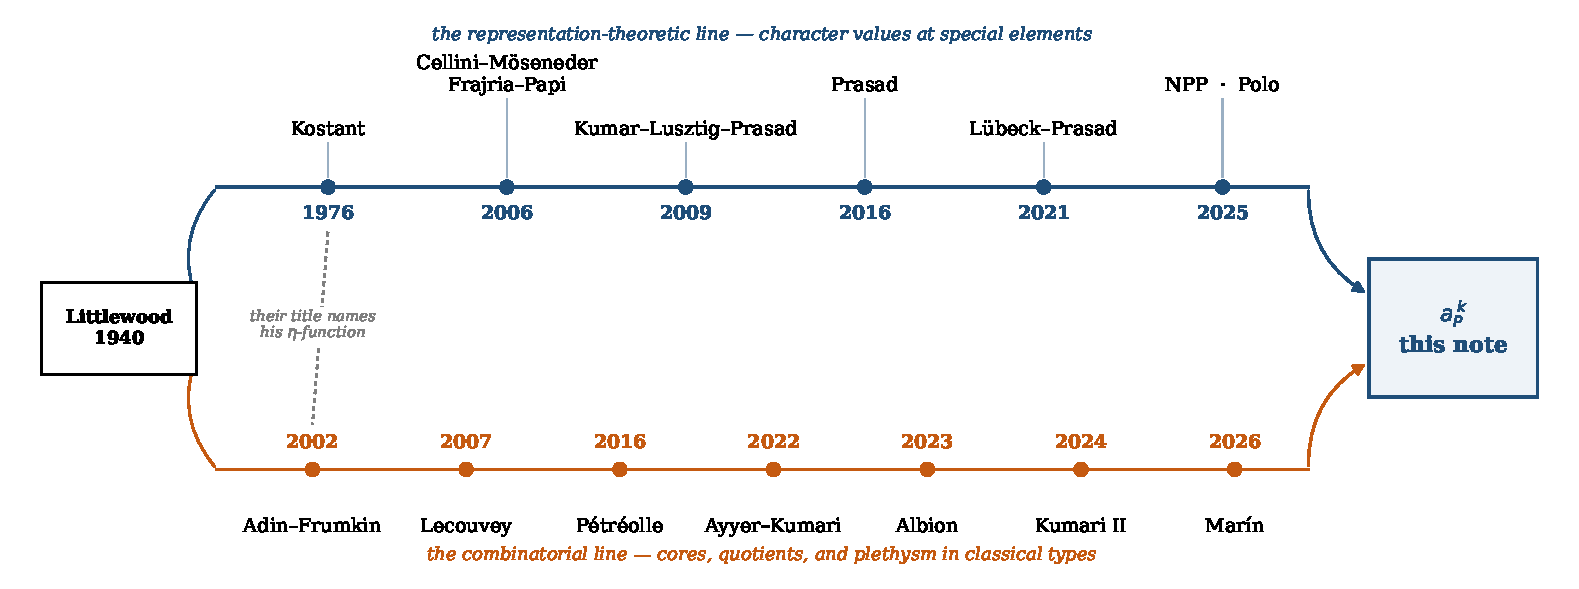
\includegraphics[width=\textwidth]{fig_map.pdf}
\caption{\textbf{Las dos líneas.} El eje es el tiempo y cada nodo lleva un nombre y su año de
\emph{publicación}, que son los de la bibliografía de abajo. Arriba, valores de caracteres en
elementos especiales: Kostant \cite{Kostant76} fija $a_Q$ y $a_P$ y demuestra que los valores son
$\{0,\pm1\}$; Cellini--Möseneder Frajria--Papi \cite{CMP06} evalúan el carácter en $a_P$ sin más;
Kumar--Lusztig--Prasad \cite{KLP09} hacen de \emph{torcido} y \emph{plegado} la misma palabra;
Prasad \cite{Prasad16,Prasad16b} da la geometría de $\rho$ y el criterio de residuos en $\GL_n$;
Lübeck--Prasad \cite{LP20} lo llevan a $S_{2n}$ y $B_n$; y en 2025 llegan NPP \cite{NPP25} y Polo
\cite{Polo25}. Abajo, el lado combinatorio: núcleos en tipo $A$ \cite{AF02}; el $\ell$-cociente en
tipos clásicos por pletismos \cite{Lec07a,Lec07b}; la identidad de Macdonald de tipo $\widetilde C$
\cite{Petreolle15}; y los caracteres torcidos por raíces de la unidad \cite{AK22,Alb23,Kum24}.
Littlewood 1940 queda fuera de las dos porque alimenta a las dos, y la caja de la derecha es esta
nota: las dos flechas que entran en ella son las dos cosas que necesita, el elemento de arriba y el
alfabeto de abajo.
\textbf{El nodo que hay que leer primero es el de 2006.} El Corolario~3.2 de \cite{CMP06} ya es el
criterio de anulación \emph{y} el signo, en todo tipo, y en el estadístico de \emph{raíces} --- esta
recta, no la de corraíces. Todo lo que esta nota tiene que añadir empieza un paso más allá: en las
potencias $a_P^{\,k}$, donde $\rho$ deja de ser regular. En el estadístico de corraíces el criterio
es el Corolario~3.7 de \cite{NPP25}, para todo entero.
La arista de puntos es el cruce de 2002: el título de Adin--Frumkin es \emph{Rim hook tableaux and
Kostant's $\eta$-function coefficients}, un artículo combinatorio que toma sus coeficientes del de
1976, donde están definidos los dos elementos de Kostant. Las dos líneas sí se ven, y conviene ser
exacto en cuánto: \cite{NPP25} cita a Ayyer--Kumari; los artículos de Kumari están motivados por una
conjetura de Wagh y Prasad; y Ayyer--Kumari \cite{AK22} abren diciendo que Littlewood y Prasad
hicieron sus factorizaciones \emph{«motivated by a celebrated result of Kostant»}. Así que la
conexión Prasad--Kostant está por escrito en los dos lados. Lo que \emph{no} está en ninguno es la
identificación de la \S\ref{sec:alph}: $a_P^{\,k}$ como $d\cdot\mu_q$ menos dos letras, leído en la
recta de $\rho$. \ver{figs.py}}
\label{fig:map}
\end{figure}

\section{Normalizaciones, y de qué elemento se trata}\label{sec:norm}

Toda la nota gira sobre un eje --- raíces contra corraíces ---, así que las normalizaciones se fijan
primero, y con más cuidado del que el objeto parece pedir.

Sea $G$ simple y simplemente conexo con toro maximal $T$, raíces $\Phi$, raíces positivas $\Phi^+$ y
$\rho$ la semisuma de $\Phi^+$. Normalícese la forma invariante de modo que las raíces cortas tengan
$(\alpha,\alpha)=2$, y escríbase $\rho^\sharp$ para el vector de $\mathfrak t$ que la forma
identifica con $\rho$. Para un parámetro real $\theta$ póngase
\begin{equation}\label{eq:gtheta}
g_\theta \;=\; \exp\bigl(2\pi i\,\theta\,\rho^\sharp\bigr)\;\in\;T ,
\end{equation}
de modo que un peso $\mu$ toma en $g_\theta$ el valor $e^{2\pi i\theta(\mu,\rho)}$. En todo lo que
sigue $\theta=p/q$ en forma irreducible, y \textbf{$q$ es el denominador del parámetro}, que es el
entero módulo el cual se toma cada recuento.

\begin{keybox}
\textbf{$q$ no tiene por qué ser el orden de $g_\theta$, ni $\rho^\sharp$ un cocarácter.} En $A_1$
con $(\alpha,\alpha)=2$ se tiene $\rho=\omega$ y $(\omega,\rho)=\tfrac12$, así que la representación
estándar tomaría los valores $z^{\pm1/2}$: la aplicación $z\mapsto\rho(z)$ es un cocarácter del grupo
adjunto, no de $SL_2$. En concreto $g_{1/q}=\operatorname{diag}(e^{\pi i/q},e^{-\pi i/q})$ tiene
orden $2q$ en $SL_2$, no $q$. Nada de lo que sigue se ve afectado --- todo enunciado es sobre el
\emph{denominador} $q$ ---, pero los dos no deben confundirse: para
$\operatorname{diag}(i,-i)$, de orden $4$, el carácter estándar se anula, y un recuento hecho con
$q=4$ en esta normalización no lo ve.
\end{keybox}

\noindent \textbf{En tipo $C$}, que es donde transcurre todo a partir de la \S\ref{sec:cap}, no hace
falta ese cuidado. En $\Sp(2m)$ se tiene $\rho=(m,m-1,\dots,1)$ en las coordenadas estándar, el
subgrupo $\theta\mapsto g_\theta$ tiene autovalores $e^{\pm2\pi i\theta j}$, y con
\[
t=2m+2,\qquad d=\gcd(k,t),\qquad q=t/d,\qquad p=k/d,
\]
el segundo elemento de Kostant es $a_P=g_{1/t}=\rho(\zeta_t)$, y
\[
a_P^{\,k}=\rho(\zeta_t^{\,k})=\rho(\xi_q),\qquad \xi_q=\zeta_t^{\,k}\ \text{raíz primitiva
$q$-ésima de la unidad},
\]
así que evaluar en $\xi_q$ la especialización principal \eqref{eq:ps} de la \S\ref{sec:crit}
calcula $\chi_\lambda(a_P^{\,k})$: ése es todo el puente, y es el único sitio donde el parámetro y el
elemento quedan atados. La relación $q\mid 2m+2$ pertenece al tipo $C$ y a las potencias de $a_P$;
no forma parte de ningún enunciado general de más abajo. \emph{Comprobado en los $140$ pares con $2\le m\le11$, $1\le k\le14$: el espectro de
$g_{p/q}$ es el alfabeto de la Proposición~\ref{prop:alph} y $\zeta_t^{\,k}$ tiene orden exactamente
$q$.} \ver{revision\_52\_bisagra.py}

\section{El criterio, y qué parte de él ya está impresa}\label{sec:crit}

\subsection*{La identidad}

La especialización principal clásica se escribe habitualmente en la recta de $\rho^\vee$, con el
estadístico de corraíces $\langle\lambda+\rho,\alpha^\vee\rangle$. Escrita en la recta de $\rho$
dice
\begin{equation}\label{eq:ps}
\boxed{\;\chi_\lambda(g_\theta)\;=\;e^{-2\pi i\theta(\lambda,\rho)}\prod_{\alpha>0}
\frac{1-e^{2\pi i\theta(\lambda+\rho,\,\alpha)}}{1-e^{2\pi i\theta(\rho,\,\alpha)}}\;}
\end{equation}
con el estadístico de \emph{raíces}. No hay que creérsela: con $\ell=\lambda+\rho$,
$\sum_w\epsilon(w)z^{(w\ell,\rho)}=\sum_w\epsilon(w)z^{(w\rho,\ell)}$ porque
$(w\ell,\rho)=(\ell,w^{-1}\rho)$ y $\epsilon(w)=\epsilon(w^{-1})$; la identidad del denominador de
Weyl convierte el miembro derecho en
$z^{(\rho,\ell)}\prod_{\alpha>0}(1-z^{-(\ell,\alpha)})$; y dividiendo por el mismo cálculo en
$\ell=\rho$ sale \eqref{eq:ps}. Lo único que cambia respecto de la forma habitual es en cuál de las
dos rectas se está --- que es precisamente el eje que separa a los dos elementos de Kostant.
\emph{Comprobada contra el bialternante en la recta de $\rho$ para $m=2,3,4$ hasta $10^{-12}$.}
\ver{revision\_47\_verificacion.py}

\subsection*{El recuento}

\begin{theorem}[el criterio]\label{thm:crit}
Sea $\lambda$ dominante, $\ell=\lambda+\rho$, $\theta=p/q$ irreducible, y póngase
\[
N_q(x)=\#\{\alpha>0:\ q\mid(x,\alpha)\},\qquad r_q=N_q(\rho) .
\]
Entonces $N_q(\ell)\ge r_q$ para todo $\lambda$, y
\begin{equation}\label{eq:crit}
\boxed{\;\chi_\lambda(g_{p/q})\neq0 \iff N_q(\ell)=r_q\;}
\end{equation}
\end{theorem}

\begin{proof}
Cada factor $1-z^{r}$ de \eqref{eq:ps} tiene un cero simple en una raíz primitiva $q$-ésima de la
unidad exactamente cuando $q\mid r$, así que en $z=e^{2\pi ip/q}$ el numerador se anula a orden
$N_q(\lambda)$ y el denominador a orden $r_q$. Un carácter no tiene polos, luego el primer orden es
al menos el segundo; y el límite es no nulo exactamente cuando coinciden.
\end{proof}

\noindent Nada en esa demostración usa $q\mid 2m+2$, ni el tipo $C$, ni que $p=1$: el enunciado es
sobre toda la recta $\theta\mapsto g_\theta$, en todo parámetro racional. Las potencias de $a_P$ en
$\Sp(2m)$ son la subfamilia $q\mid 2m+2$. \emph{Medido sobre $\mathbf{27\,183}$ pesos dominantes en
$\Sp(2m)$, $m=2,\dots,6$ y $q=2,\dots,14$, sin excepción --- y $\mathbf{19\,986}$ de ellos tienen
$q\nmid t$. La condición ingenua «alguna raíz divide», corrida como señuelo sobre los mismos pesos,
falla $7\,968$ veces, así que la prueba discrimina; ningún valor quedó numéricamente ambiguo.}
\ver{rho\_line\_any\_q.py}

\subsection*{Lo que ya está impreso, y lo que no}

\begin{keybox}
\textbf{El mismo recuento, en la otra recta, es el Corolario~3.7 de \cite{NPP25}}, y hay que leerlo
antes de leer lo de arriba como nuevo. En su notación, para todo entero positivo $m$ y todo
$\lambda$ dominante:
\[
\#\{\alpha\in\Phi^+ : m\mid\langle\rho,\alpha^\vee\rangle\}\;\le\;
\#\{\alpha\in\Phi^+ : m\mid\langle\lambda+\rho,\alpha^\vee\rangle\},
\]
\emph{y $\Theta_\lambda(\rho^\vee(e^{2\pi i/m}))\neq0$ si y sólo si esa desigualdad es una igualdad.}
Su Proposición~3.8 lee después los dos miembros como dimensiones de centralizadores en el grupo
dual, y atribuye la minimalidad a Serre.

\smallskip
\textbf{Así que la diferencia es el estadístico, y por tanto el elemento.} El
Teorema~\ref{thm:crit} es el recuento sobre $(\,\cdot\,,\alpha)$ --- la recta de $\rho$, donde vive
$a_P$ --- y el suyo es el recuento sobre $\langle\,\cdot\,,\alpha^\vee\rangle$ --- la recta de
$\rho^\vee$, donde vive el elemento de Coxeter. \textbf{En los tipos simplemente enlazados los dos
enunciados coinciden} bajo la normalización de la \S\ref{sec:norm}, y allí el
Teorema~\ref{thm:crit} es suyo. Se separan exactamente en los no simplemente enlazados, que es
exactamente donde se separan $a_P$ y $a_Q$, y ése es el caso del que trata esta nota.
\end{keybox}

\noindent Lo que queda, entonces, y es el resto de la nota: la identificación del alfabeto
(\S\ref{sec:alph}), la traducción a capacidades en tipo $C$ (\S\ref{sec:cap}), el valor exacto con su
signo (\S\ref{sec:valor}), el módulo y su lema (\S\ref{sec:modulo}), la factorización en
dimensiones (\S\ref{sec:dims}), los recuentos
(\S\ref{sec:cuenta}) y $G_2$ (\S\ref{sec:g2}).

\section{Por qué las dos tablas se parecen: el alfabeto}\label{sec:alph}

\noindent\emph{Dos tablas escritas en dos literaturas que no se citan tienen la misma forma. ¿Es un parecido, o hablan del mismo objeto?}

Se parecen porque los alfabetos son el mismo objeto. Éste es el único sitio donde puedo sustituir el
parecido por una identidad, y es elemental.

\begin{proposition}\label{prop:alph}
Sean $t=2m+2$, $d=\gcd(k,t)$ y $q=t/d$. Como multiconjunto, el alfabeto simpléctico de $a_P^k$, es
decir $A=\{\zeta^{\pm jk}: j=1,\dots,m\}$ con $\zeta$ de orden $t$, cumple
\[
A \;=\; d\cdot\mu_q \;-\; 2\cdot\{1\} \quad (d \text{ par}),
\qquad
A \;=\; d\cdot\mu_q \;-\;\{1\}-\{-1\} \quad (d \text{ impar}).
\]
\end{proposition}

\begin{proof}
Como $t=2m+2$, los exponentes $\{\pm j : j=1,\dots,m\}$ son exactamente
$\mathbb{Z}/t\smallsetminus\{0,t/2\}$. La aplicación $e\mapsto\zeta^{ke}$ factoriza por
$\mathbb{Z}/q$, porque $\zeta^k$ tiene orden $q$, y cada residuo módulo $q$ es imagen de exactamente
$d$ elementos de $\mathbb{Z}/t$; luego $\{\zeta^{ke}: e\in\mathbb{Z}/t\}=d\cdot\mu_q$. Queda quitar
los dos exponentes excluidos. Para $e=0$ el elemento es $1$. Para $e=t/2=dq/2$: si $d$ es par esto es
$\equiv 0 \pmod q$ y el elemento vuelve a ser $1$; si $d$ es impar entonces $q$ es par, porque
$dq=t$ lo es, y $dq/2\equiv q/2$, así que el elemento es $-1$.
\end{proof}

\noindent Antes de las consecuencias, una atribución que va aquí. El alfabeto \emph{sin borrar}
$d\cdot\mu_q$ tampoco es terreno virgen en mi lado del mapa: Ayyer y Kumari \cite{AK22} tratan
exactamente el carácter simpléctico de $\Sp_{2t'n}$ en $\omega^j x_i$ --- siendo $t'$ su orden de
$\omega$ y $n$ su número de variables --- que en $x_i=1$ es $\mu_{t'}$ con multiplicidad $2n$,
contando cada autovalor con su recíproco. Dan tanto un criterio de anulación como una factorización
en caracteres de grupos clásicos menores. Su multiplicidad es por tanto siempre par, y no hay
borrado. Así que el
alfabeto grande está hecho a los dos lados del mapa; lo que no está hecho son los dos puntos.

Dos consecuencias, y la primera es el diccionario.

\begin{keybox}
El alfabeto del Teorema~2 de \cite{Prasad16b} en $t=1$ --- el $t$ de ese artículo, el elemento de $\GL_m$, no el $t=2m+2$ de esta
nota --- es $\mu_n$ con multiplicidad $m$. El mío es $\mu_q$ con
multiplicidad $d$, \emph{menos dos puntos}. Así que el $m$ de allí es el $d$ de aquí y el $n$ de allí es el $q$ de aquí --- no por
analogía, sino porque los multiconjuntos son el mismo --- y los dos puntos que faltan son
puntos fijos de $w\mapsto w^{-1}$ --- una copia de cada uno de los dos si $d$ es impar, dos copias
del único $w=1$ si $d$ es par.
\end{keybox}

\noindent Eso deja resueltas las tres primeras filas de la tabla de la página~1, y dice exactamente
de dónde sale la fila naranja: la diferencia entre los dos criterios es la diferencia entre los dos
alfabetos, que son dos puntos. Lo que \emph{no} hace es calcular el efecto de quitarlos --- borrar
dos letras es un problema de eliminación --- una ramificación simpléctica en sentido literal sólo
si $d$ es par, por la razón que da la segunda ficha de abajo --- y no lo he llevado a cabo --- pero resultó no hacer falta para la
anulación, que el Corolario~\ref{conj:cap} cierra por otra vía. Sigue siendo la entrada natural para
el \emph{valor}, y la \S\ref{sec:cierre} vuelve sobre ella.

La segunda consecuencia es la función generatriz, que es lo que hace todo calculable:
\[
H(z)=\frac{(1-z)^2}{(1-z^q)^d}\quad (d\text{ par}),
\qquad
H(z)=\frac{1-z^2}{(1-z^q)^d}\quad (d\text{ impar}),
\]
de modo que los $h_n$ son enteros --- con soporte en los residuos $0,1,2$ módulo $q$ si $d$ es par
y en $0,2$ si $d$ es impar --- y todo determinante de esta nota es exacto. Las dos afirmaciones comprobadas contra el alfabeto calculado directamente, y la
versión con la paridad de $d$ invertida acierta en $0$ de $72$ casos. \ver{aP\_alfabeto.py}

\noindent Qué \emph{es} el borrado, geométricamente, depende de la paridad de $d$; y ha hecho falta
una versión equivocada de este párrafo para verlo.

\begin{keybox}
\textbf{Sin condiciones:} el elemento de $\GL_t$ de \cite{Prasad16b} tiene alfabeto $d\cdot\mu_q$, y el alfabeto de
$a_P^{\,k}$ en $\Sp(t-2)$ es ése con exactamente dos letras borradas --- si $d$ es par, dos copias
del punto fijo $1$; si $d$ es impar, una copia de cada uno de los dos puntos fijos $1$ y $-1$.

\smallskip
\textbf{Sólo con $d$ par} puede leerse eso como quitar un plano simpléctico. Con $d$ impar no puede:
entonces $q$ es par, los autovalores $1$ y $-1$ aparecen en $d\cdot\mu_q$ con multiplicidad $d$, que
es impar, y $\det(d\cdot\mu_q)=(-1)^{d}=-1$, de modo que \emph{ningún} elemento de $\Sp(t)$ tiene ese
espectro; ni $\{1,-1\}$, de determinante $-1$, es un plano simpléctico. El caso mínimo es $d=1$,
$q=6$: el producto sobre $\mu_6$ vale $-1$, así que $\mu_6$ no es espectro en $\Sp(6)$ --- mientras
que $\mu_6\smallsetminus\{1,-1\}$ sí lo es en $\Sp(4)$.
\end{keybox}

\noindent De modo que los dos lados están unidos por una identidad de alfabetos, no siempre por una
identidad de elementos, y $d$ impar --- que incluye al propio $a_P$ --- es justo donde falla la
imagen geométrica. Eso además quita la explicación fácil de las capacidades: no se pueden achacar sin
más a «los dos puntos fijos», porque con $d$ par interviene un solo punto fijo, dos veces.

Lo que eso deja pendiente ya no es vago. Quitar las dos letras actúa sobre la función
generatriz como un solo factor, así que al nivel de los $h_n$ es una diferencia finita:
\[
h^{A} = (1-S)^2\,h' \quad (d \text{ par}), \qquad h^{A} = (1-S^2)\,h' \quad (d \text{ impar}),
\]
donde $h'_n=\mathbf{1}_{q\mid n}\binom{n/q+d-1}{d-1}$ son los suyos --- el indicador importa, porque $h'_n=0$ salvo que $q\mid n$ --- y $S$ es el desplazamiento. De modo que el hueco
entre esta nota y una derivación es exactamente una pregunta: \emph{¿qué le hace una diferencia
segunda de la sucesión $h$ al determinante de Jacobi--Trudi?} La tomé por una obstrucción, y no lo
es: sale como un producto de operadores de una variable, en dos líneas, y la \S\ref{sec:cierre} lo
hace. Lo que eso sigue dejando --- la cancelación entre los determinantes desplazados --- es donde
esta nota se para.


\section{Qué puntos de la recta dan respuestas enteras}\label{sec:clasif}

\noindent\emph{La Proposición~\ref{prop:alph} leyó el alfabeto de $a_P^{\,k}$ como un múltiplo entero
de $\mu_q$ menos dos letras. Todo punto de la recta tiene alfabeto, y en casi todos no tiene esa
forma. ¿Qué tienen de especial los que sí?}

\smallskip
\noindent En general, con $m=uq+v$, el alfabeto es $2u\cdot\mu_q$ con un segmento
$\{\pm1,\dots,\pm v\}$ añadido, y la Proposición~\ref{prop:alph} es el caso en que ese segmento
cierra. La pregunta buena no es cuáles se ven limpios, sino a cuáles la aritmética no puede
distinguir de sus propios conjugados de Galois --- y eso resulta ser un enunciado sobre los
caracteres, no sobre la notación: si son \emph{números enteros}. El criterio de la \S\ref{sec:crit}
vale en todo punto racional, así que nada hasta aquí ha impuesto la familia $q\mid 2m+2$ que el
resto de esta nota evalúa. Esto es lo que la señala.

\begin{theorem}[qué denominadores dan valores enteros]\label{thm:clasif}
Sean $m\ge2$ y $\gcd(p,q)=1$. Entonces $\chi_\lambda(g_{1/q})\in\mathbb{Z}$ para \emph{todo} peso
dominante $\lambda$ si y sólo si se cumple al menos una de
\[
q\mid 2m,\qquad q\mid 2m+1,\qquad q\mid 2m+2,\qquad q=6 \text{ y } m\equiv1 \!\!\pmod 3 ;
\]
y en ese caso $g_{p/q}$ es conjugado de $g_{1/q}$ para todo $p$ coprimo con $q$, de modo que ningún
valor de carácter depende del numerador.
\end{theorem}

\noindent La palabra \emph{todo} es la que sostiene el enunciado. No se clasifica cuándo un carácter
concreto sale entero --- eso pasa por toda la recta --- sino cuándo salen enteros todos a la vez.

\begin{proof}[El argumento, que no mira ningún peso]
Supóngase que todo $\chi_\lambda(g_{1/q})$ es entero. Las potencias exteriores
$\Lambda^j\mathbb{C}^{2m}$ son sumas directas de irreducibles --- no irreducibles ellas mismas ---,
así que sus caracteres son
combinaciones enteras de los $\chi_\lambda$ y por tanto también enteros; y esos caracteres son los
coeficientes del polinomio característico de $g_{1/q}$ actuando en $\mathbb{C}^{2m}$; luego ese polinomio está en
$\mathbb{Z}[X]$, y las multiplicidades de sus raíces son constantes en las órbitas de Galois. Al
revés, si el espectro se lleva a sí mismo por todo $\xi_q\mapsto\xi_q^{\,p}$, entonces $g_{p/q}$ y
$g_{1/q}$ tienen el mismo espectro y son conjugados en $\Sp(2m)$; los valores de los caracteres son
entonces enteros algebraicos fijos por el grupo de Galois de $\mathbb{Q}(\xi_q)$, o sea enteros
racionales.

Lo que queda es elemental. Escríbase $m=uq+v$ con $0\le v<q$ y $a=\lfloor(q-1)/2\rfloor$. El
espectro de la natural es $\{\xi_q^{\pm j}: j=1,\dots,m\}$, que como multiconjunto de $\mu_q$ es
\[
2u\cdot\mu_q \;+\;\{\pm1,\dots,\pm v\} ,
\]
y el primer sumando ya es estable por sí solo. Así que la pregunta es cuándo lo es el segmento
$\{\pm1,\dots,\pm v\}$, y eso es una cuestión de residuos y de nada más. La suficiencia es
inmediata para $v=0$, $v=a$, $v=q-1$ y, con $q$ par, $v=q/2$: cada uno de esos segmentos va a sí
mismo por todo $\xi_q\mapsto\xi_q^{\,p}$. La necesidad es el paso que hay que argumentar.

Escribamos $A_v=\sum_{j=1}^{v}(\xi_q^{\,j}+\xi_q^{-j})$. Si el segmento es estable, $A_v$ queda
fijo por todo el grupo; sólo se usa esa dirección, y se usa por contrarrecíproco. Una vuelta completa suma cero, luego
$A_v+A_{q-1-v}=-2$ y $\mathbb{Q}(A_v)=\mathbb{Q}(A_w)$ con $w=\min(v,q-1-v)$; los cuatro segmentos
recién listados son $w=0$ y $w=a$, así que sólo queda $1\le w<a$. Ahí ponemos
$\beta_w=1+A_w=\sum_{j=-w}^{w}\xi_q^{\,j}$, un núcleo de Dirichlet, cuyos conjugados son
\[
  \sigma_p(\beta_w)=\frac{\sin\bigl((2w+1)\pi p/q\bigr)}{\sin(\pi p/q)} .
\]
Para $q\ge4$, $2\le N\le q-2$ y $1\le r\le q-1$ con $r\neq1,q-1$, se tiene la desigualdad
\emph{estricta}
\[
  \Bigl|\frac{\sin(N\pi r/q)}{\sin(\pi r/q)}\Bigr|
  \;<\;\frac{\sin(N\pi/q)}{\sin(\pi/q)} .
\]
En efecto, sustituir $N$ por $n=\min(N,q-N)$ no cambia ningún módulo; en $0<x<\pi/n$ la función
$f(x)=\sin(nx)/\sin x$ es positiva y estrictamente decreciente, porque $f'/f=n\cot(nx)-\cot x<0$ ya
que $t\cot t$ decrece en $(0,\pi)$; y en $\pi/n\le x\le\pi/2$ se tiene
$|f(x)|\le 1/\sin(\pi/n)<1/\sin(\pi/2n)=f(\pi/2n)\le f(\pi/q)$. Tomando $N=2w+1$, que cae en ese
rango justo cuando $1\le w<a$, los únicos automorfismos que fijan $\beta_w$ son la identidad y la
conjugación compleja; luego $\mathbb{Q}(\beta_w)=\mathbb{Q}(\xi_q+\xi_q^{-1})$, que es
$\mathbb{Q}$ sólo cuando $\varphi(q)=2$. Dentro de este rango eso deja $q=6$, $w=1$ --- los dos
segmentos $(q,v)=(6,1)$ y $(6,4)$. Traducir los residuos que sobreviven a divisibilidades da las
cuatro condiciones.
\end{proof}

\noindent \emph{Medido sobre $\mathbf{11\,800}$ pares $(m,q)$ con $q\le60$ y $m\le200$: la condición
de divisibilidad y la estabilidad de Galois del espectro coinciden sin excepción. Y sobre los $44$
pares con $m\le5$, $q\le12$ la misma coincidencia se da contra los caracteres mismos, calculados a
$40$ dígitos como límite de la forma con senos y contrastada su integridad --- de modo que la cadena
que va de la aritmética a los valores queda comprobada en sus dos junturas.} \ver{galois.py}

\begin{keybox}
\textbf{Las potencias de $a_P$ son la tercera familia.} $q\mid 2m+2$ es exactamente la condición
$q\mid t$, así que de la \S\ref{sec:valor} en adelante se evalúa una de las cuatro. Las otras tres
son puntos de la misma recta donde todo carácter es entero y $a_P$ no pinta nada: en $\Sp(10)$ con
$q=5$, donde $5\mid m$, o en $\Sp(6)$ con $q=7$, donde $7\mid 2m+1$ y todo valor es $0$ o $\pm1$
aunque el orden de $a_P$ sea $8$.

\smallskip
\textbf{Y ser entero no es la cancelación de la \S\ref{sec:modulo}.} Las dos se confunden con
facilidad y son distintas. En $\Sp(4)$ con $q=4$ --- que está en la lista, porque $4\mid 2m$ ---
tómese $\lambda=(1,0)$. Entonces $Z_4(\ell)/Z_4(\rho)=1$, mientras que
\[
\chi_{(1,0)}(g_{1/4})=-2 .
\]
Todo carácter en ese punto es entero, y el factor no nulo tiene módulo $2$, no $1$. \emph{Sobre los
$(m,q)$ con $q\le40$, $m\le120$, los puntos donde el factor se cancela son $\mathbf{1119}$ y están
contenidos en la lista de arriba; la lista tiene $\mathbf{177}$ más, y ésos son exactamente los
puntos donde el valor es entero pero la fórmula de esta nota necesita un corrector.}
\ver{dos\_clasif.py}
\end{keybox}

\section{Capacidades en tipo $C$}\label{sec:cap}

\noindent\emph{El criterio cuenta raíces. En las coordenadas del tipo $C$, ¿qué está contando --- y se puede ver de un vistazo si un peso pasa?}

El Teorema~\ref{thm:crit} es un enunciado sobre un sistema de raíces. En las coordenadas del tipo
$C$ se vuelve una regla sobre cubos, y esa traducción es lo que hace calculable todo lo que sigue.


\noindent\textbf{(iv) Lo mismo en las coordenadas del tipo $C$.} En $C_m$ las raíces positivas son $e_i-e_j$,
$e_i+e_j$ y $2e_i$, luego agrupando los $\ell_i$ en clases plegadas de ocupación $n_c$,
\[
N_q(\ell)=\sum_{c\ \text{no fija}}\binom{n_c}{2}\;+\;\sum_{f\ \text{fija}}n_f^{\,2},
\]
porque en una clase no fija cada pareja aporta exactamente una de $e_i\pm e_j$, y en una fija aporta
las dos, más el $2e_i$ de cada índice: $2\binom n2+n=n^2$. El coste marginal de una fila más es
entonces $0,1,2,\dots$ en una no fija y $1,3,5,\dots$ en una fija, de modo que las plazas que cuestan
menos que $d$ son exactamente $d$ por clase no fija y $\lfloor d/2\rfloor$ por clase fija. Ahora se
cuentan. Si $d$ es impar hay exactamente $m$ de esas plazas, así que alcanzar el mínimo $r_q$ obliga
a ocuparlas todas, y cualquier desbordamiento cambia una plaza de coste $<d$ por otra de coste
$\ge d$. Si $d$ es par hay exactamente $m+1$; toda última plaza admisible cuesta $d-1$, así que
omitir cualquiera de ellas da el mismo mínimo, mientras que pasarse de una capacidad vuelve a costar
estrictamente más. Así que $N_q(\lambda)=r_q$ si y sólo si no se rebasa ninguna capacidad, y con el
Teorema~\ref{thm:crit} eso es:

\begin{corollary}[capacidad, tipo $C$]\label{conj:cap}
$\chi_\lambda(a_P^k)\neq0$ si y sólo si cada clase plegada módulo $q$ recibe a lo sumo $d$ de los
$\ell_i$, y a lo sumo $\lfloor d/2\rfloor$ si la clase es fija.
\end{corollary}

\noindent Ésa es la regla que había medido, y la fila naranja de la tabla de la página 1.
\emph{El Teorema~\ref{thm:crit} y el Corolario~\ref{conj:cap} se comprobaron los dos contra el
evaluador exacto en las mismas $31$ combinaciones: $100\%$ en todas.}
\ver{revision\_47\_verificacion.py}

\subsection*{De dónde sale la única unidad de holgura}

El criterio de \cite{Prasad16b} es una igualdad y el de aquí una desigualdad. Un diccionario con una
entrada rota no es un diccionario, así que ésta es la parte que más quería cerrar, y fue lo primero
que supe demostrar: antes de que existiera el Corolario~\ref{conj:cap}, esto era todo lo que sabía.
Leído ahora, es el aspecto que tiene ese corolario desde el lado de \cite{Prasad16b}.

\begin{proposition}\label{prop:slack}
En tipo $A$ el número de filas es igual a la capacidad total. En tipo $C$, con $m=dq/2-1$ filas, la
capacidad total es $dq/2$ si $d$ es par y $dq/2-1$ si $d$ es impar.
\end{proposition}

\begin{proof}
En tipo $A$ hay $mn$ beta-números y $n$ clases de capacidad $m$: total $mn$, el número de filas. En
tipo $C$ las clases plegadas son $\lfloor q/2\rfloor+1$, una fija si $q$ es impar y dos si $q$ es par.
Si $q$ es par, la capacidad es $d(q/2-1)+2\lfloor d/2\rfloor$, que vale $dq/2$ para $d$ par y
$dq/2-1$ para $d$ impar. Si $q$ es impar entonces $d$ es par, porque $dq=t$ es par, y la capacidad es
$d(q-1)/2+\lfloor d/2\rfloor=dq/2$.
\end{proof}

\begin{keybox}
Cuando $d$ es \textbf{impar} la capacidad se satura exactamente, «a lo sumo» y «exactamente» dicen lo
mismo, y el criterio \emph{es} la igualdad de \cite{Prasad16b}. Cuando $d$ es \textbf{par} sobra
exactamente una unidad. Y sobra entera de las clases fijas, que llevan $\lfloor d/2\rfloor$ en vez de
$d$. Así que la desigualdad no es un debilitamiento de ese enunciado: es ese enunciado con exactamente una unidad de
holgura, y la holgura existe porque el plegado tiene puntos fijos siquiera. Los
puntos fijos existen porque el plegado es una involución.
\end{keybox}

\noindent La Figura~\ref{fig:capacity} dibuja los dos casos. Comprobado en forma cerrada
sobre los $\mathbf{2170}$ pares con $2\le m\le59$,
$1\le k\le39$ y $q\ge3$. \ver{prasad2016\_vs\_nuestro.py, \S W}

\begin{figure}[tbp]
\centering
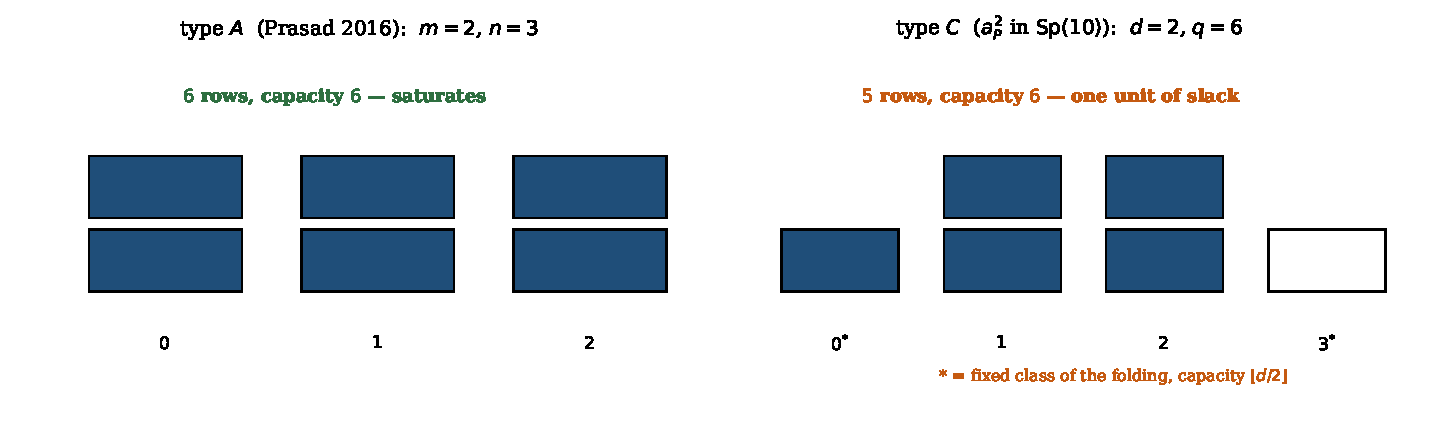
\includegraphics[width=\textwidth]{fig_capacity.pdf}
\caption{La Proposición~\ref{prop:slack}, dibujada. Izquierda, tipo $A$: las cajas se llenan exactas.
Derecha, tipo $C$ en $a_P^2$ dentro de $\Sp(10)$: las dos clases con asterisco son los puntos fijos
de la involución y llevan media capacidad, así que cinco filas van a seis cajas y una tiene que
quedarse vacía. Cuál se queda vacía no lo determina $\lambda$ de ninguna manera que yo vea.}
\label{fig:capacity}
\end{figure}


\section{El valor, con su signo}\label{sec:valor}

\noindent\emph{Hasta aquí la respuesta ha sido sí o no. Cuando es que sí, ¿cuánto vale el número?}

Escríbase, para un vector $x$ y las raíces positivas del tipo $C$,
\[
Z_q(x)\;=\;\prod_{\substack{\alpha>0\\ q\mid(x,\alpha)}}(x,\alpha)
\qquad\text{(producto vacío $=1$)},
\qquad
E_{p,q}(\lambda)\;=\;\sum_{\alpha>0}\left(
\Bigl\lfloor\tfrac{p(\ell,\alpha)}{q}\Bigr\rfloor-\Bigl\lfloor\tfrac{p(\rho,\alpha)}{q}\Bigr\rfloor
\right).
\]

\begin{theorem}[el valor, toda potencia, tipo $C$]\label{thm:signo}
En $\Sp(2m)$, para todo $k$, con $d=\gcd(k,2m+2)$, $q=(2m+2)/d$ y $p=k/d$,
\[
\boxed{\;
\chi_\lambda(a_P^{\,k})\;=\;
\begin{cases}
0, & N_q(\ell)>r_q,\\[2mm]
(-1)^{E_{p,q}(\lambda)}\,\dfrac{Z_q(\lambda+\rho)}{Z_q(\rho)}, & N_q(\ell)=r_q .
\end{cases}\;}
\]
\end{theorem}

\begin{proof}[Derivación del signo]
Como $\sum_{\alpha>0}(\lambda,\alpha)=2(\lambda,\rho)$, las fases de \eqref{eq:ps} se cancelan contra
su prefactor, y fuera de los parámetros singulares
\[
\chi_\lambda(g_\theta)\;=\;\prod_{\alpha>0}
\frac{\sin\bigl(\pi\theta(\ell,\alpha)\bigr)}{\sin\bigl(\pi\theta(\rho,\alpha)\bigr)} .
\]
Para un entero positivo $A$ con $q\nmid A$ se tiene
$\operatorname{sgn}\sin(\pi pA/q)=(-1)^{\lfloor pA/q\rfloor}$; y para $q\mid A$, escribiendo
$\theta=p/q+\varepsilon$, $\sin(\pi A\theta)=(-1)^{pA/q}\pi A\varepsilon+O(\varepsilon^3)$. Cuando
los órdenes de anulación coinciden --- que es \eqref{eq:crit} --- las potencias de $\varepsilon$ y
los factores $\pi$ se cancelan, cada factor que se anula deja su propio exponente, y todo factor deja
su signo. Recogiéndolos sale $(-1)^{E_{p,q}(\lambda)}$ y el cociente $Z_q(\ell)/Z_q(\rho)$.
\end{proof}

\noindent \emph{Esta derivación del signo no usa el tipo}, una vez fijada la normalización de la
\S\ref{sec:norm}; lo que sí lo usa es lo que abajo cierra el \emph{módulo}.

\smallskip
\noindent \textbf{El numerador $p$ se cae.} Por la Proposición~\ref{prop:alph} el alfabeto de
$a_P^{\,k}$ depende sólo de $d$ y $q$, así que $a_P^{\,k}$ y $a_P^{\,d}$ tienen el mismo espectro y
\[
\chi_\lambda(a_P^{\,k})=\chi_\lambda(a_P^{\,d}),\qquad d=\gcd(k,2m+2),
\]
de donde $E_{p,q}\equiv E_{1,q}\pmod 2$ en los pesos supervivientes. \emph{Comprobado: los dos
espectros coinciden como multiconjunto en los $32$ pares $(m,k)$ con $m\le5$.} \ver{referee2.py}
No cuesta nada dejar $p$ en el enunciado, y el lector puede tomar $p=1$ en todo.

\smallskip
\noindent \textbf{Y al signo le bastan los residuos, en orden.} Escribiendo $x_i=qh_i+r_i$ con
$0\le r_i<q$, los cocientes aportan $2\sum_i(m-i+1)h_i$ a la suma de pisos, que es par. Lo que queda
es un recuento de tres indicadores. Póngase
\[
F_q(r_1,\dots,r_m)=\#\{i:\,2r_i\ge q\}
\;+\;\#\{i<j:\,r_i<r_j\}
\;+\;\#\{i<j:\,r_i+r_j\ge q\} .
\]
Entonces, en los pesos supervivientes,
\[
\boxed{\;\operatorname{sgn}\chi_\lambda(a_P^{\,k})
=(-1)^{\,F_q(\ell\bmod q)-F_q(\rho\bmod q)}\;}
\]
\emph{Comprobado en los $\mathbf{11\,972}$ pesos supervivientes, $m=2,\dots,7$, toda potencia: sin
excepción.} \ver{referee2.py} La Figura~\ref{fig:value} enseña qué aspecto tiene esa alternancia. En
particular el signo es periódico módulo $qP$, porque
$E_{p,q}(\lambda+q\gamma)-E_{p,q}(\lambda)=2p(\gamma,\rho)$ es par. Ése es el sentido preciso en que
las ocupaciones de las clases plegadas no bastan y los cocientes completos no hacen falta:
\emph{qué} residuos aparecen, y \emph{en qué orden}.

\begin{figure}[tbp]
\centering
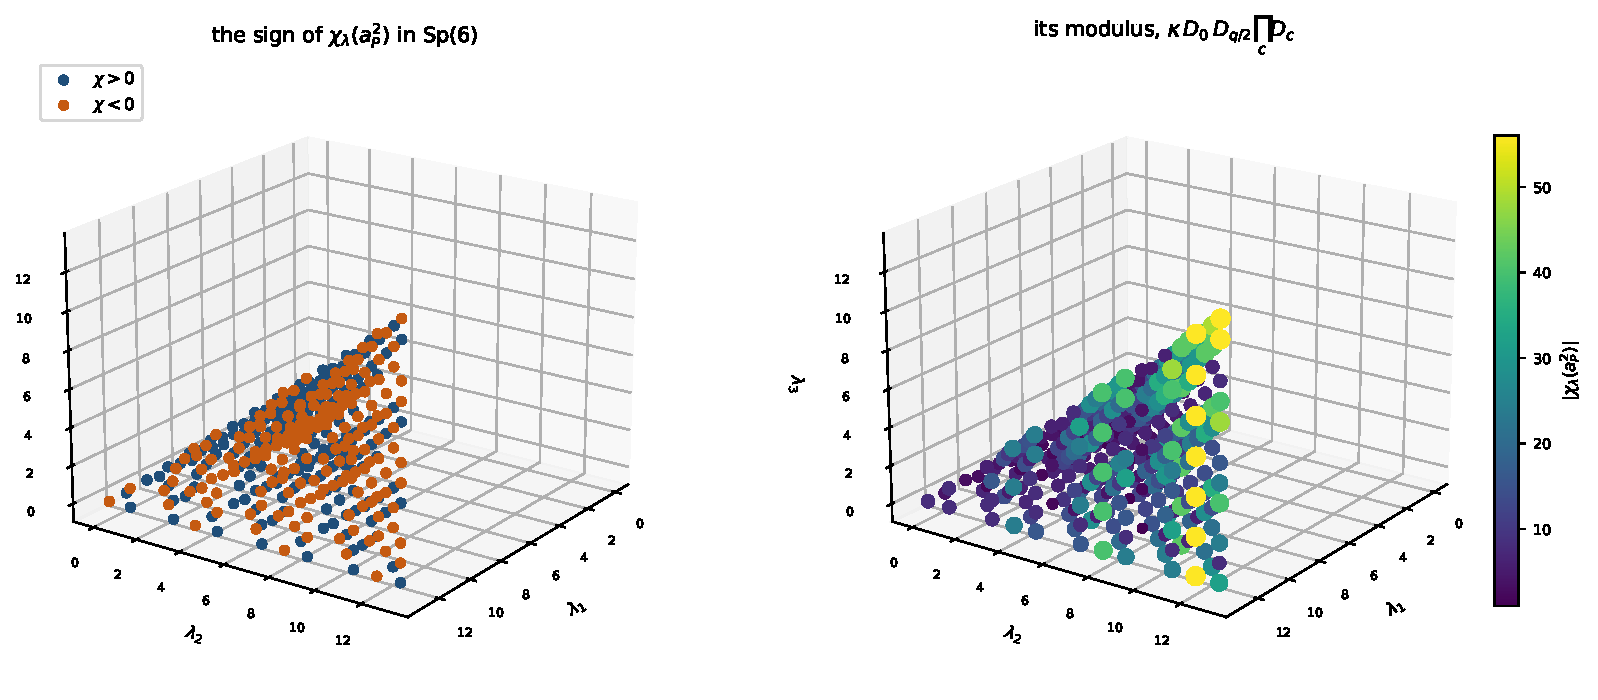
\includegraphics[width=\textwidth]{fig_value.pdf}
\caption{\textbf{El teorema, dibujado.} Cada punto es un peso superviviente de $\Sp(6)$ en $k=2$
--- o sea $d=2$, $q=4$ ---, situado en $(\lambda_1,\lambda_2,\lambda_3)$ sobre la caja
$\lambda_1\le13$; hay $\mathbf{352}$, $176$ de cada signo. Izquierda, el \emph{signo} del
Teorema~\ref{thm:signo}: alterna en láminas. Ésa es la imagen que hay detrás de los dos resultados
negativos de esta sección --- el signo no es función del patrón de ocupación, porque pesos vecinos
con las mismas clases toman los dos signos, y tampoco es ruido. Derecha, el \emph{módulo}, que por el
Teorema~\ref{thm:dims} es $\kappa\,D_0\,D_{q/2}\prod_c D_c$; va de $1$ a $\mathbf{56}$ en esta caja y
crece en la dirección en la que se llena la clase libre. \ver{fig\_value.py}}
\label{fig:value}
\end{figure}

\smallskip
\noindent \emph{Dónde se sitúa esto.} Que el carácter en un elemento de orden finito está
determinado en general no es nuevo: Kumar y Prasad \cite{KP24} calculan $ch(t,V(\lambda))$ para todo
$t\in T$ de orden finito por la fórmula de puntos fijos de Atiyah--Singer sobre $G/P$, y de ahí
deducen la asintótica de $ch(t,V(n\lambda))$. El Teorema~\ref{thm:signo} es otro tipo de enunciado
sobre una familia mucho menor: una forma cerrada elemental, en las coordenadas del tipo $C$, para los
puntos de una recta.

\begin{keybox}
\textbf{Medido.} El Teorema~\ref{thm:signo} se cumple --- valor y signo a la vez --- en
$\mathbf{18\,904}$ pesos supervivientes de $\Sp(2m)$, $m=2,\dots,8$, sobre \emph{toda} potencia, en
aritmética entera exacta: el alfabeto de $a_P^{\,k}$ da $H(z)=(1-z)^2/(1-z^q)^d$ si $d$ es par y
$(1-z^2)/(1-z^q)^d$ si es impar, luego el carácter es un determinante entero y su signo es un dato
duro. Sólo el módulo: $18\,904$ de $18\,904$. Sólo el signo: $18\,904$ de $18\,904$.
\ver{signo\_Fq.py}
\end{keybox}

\noindent \textbf{El signo no se simplifica más, y conviene decir hasta dónde se empujó.}
Escribiendo $(x,\alpha)=q\lfloor(x,\alpha)/q\rfloor+\bigl((x,\alpha)\bmod q\bigr)$ y usando
$\sum_{\alpha>0}(x,\alpha)=2(x,\rho)$, $E_{p,q}$ se convierte en $2p(\lambda,\rho)/q$ corregido por
los residuos; y la afirmación (B) de más abajo dice que los residuos de $\ell$ y los de $\rho$
coinciden \emph{salvo} $r\leftrightarrow-r$. Si coincidieran sin más, la corrección se anularía y el
signo sería $(-1)^{2p(\lambda,\rho)/q}$. No coinciden: \emph{sobre $11\,972$ pesos supervivientes ese
candidato ni siquiera es entero en $6\,800$ de ellos, y entre los demás tiene la paridad equivocada
$1\,068$ veces.} \ver{simplificaciones.py} El plegado hace trabajo real en el signo, y los pisos son
la única forma encontrada aquí que lo aguanta.

\smallskip
\noindent \textbf{Por qué el signo no salió buscando una paridad.} Antes de escribir la forma con
senos, el signo se buscó como combinación lineal sobre $\mathrm{GF}(2)$ de quince estadísticos
naturales --- las clases que toman cada rama de $\mp$, la paridad de los cocientes
$\lfloor\ell_i/q\rfloor$, la de las filas dobladas, la de $|\lambda|$, la de $(\lambda,\rho)$, la de
las inversiones de la palabra de clases, y otros. El sistema sobre $2\,582$ pesos con $m\le6$ es
\emph{incompatible}: ningún subconjunto sirve. Tampoco es el signo función del patrón de ocupación
--- de los $32$ patrones que aparecen, ninguno lleva signo constante, y el testigo mínimo es
$\lambda=(1,0)$ contra $\lambda=(1,1)$ en $\Sp(4)$ con $k=2$: mismas clases, mismo módulo $2$,
y caracteres $-2$ y $+2$. \emph{$E_{p,q}$ no estaba entre esos quince y no podía estarlo: son
paridades de cantidades naturales, y $E_{p,q}$ es una suma de pisos --- que sí tiene forma de
recuento, el $F_q$ de arriba, pero no de los suyos.} Eso es lo que compra la forma con senos. \ver{sign\_k2.py}

\section{El módulo, y el lema del que dependía}\label{sec:modulo}

\noindent\emph{El signo ya está. De la fórmula del valor queda un cociente de dos productos de enteros: ¿por qué los factores que \emph{no} se anulan no aportan nada?}

La mitad del módulo del Teorema~\ref{thm:signo} vale la pena enunciarla aparte, porque vale más
allá del tipo $C$ y porque es como se llegó a ella. En $k=2$ toma la forma de un factor por clase:

\begin{theorem}[valor, $k=2$, valor absoluto]\label{conj:val}
Para $k=2$, \textbf{y para $\lambda$ que cumpla las capacidades del Corolario~\ref{conj:cap}}:
agrúpense los $\ell_i$ por clase plegada. Entonces
\[
\boxed{\;|\chi_\lambda(a_P^k)| \;=\; \prod_{\text{clases}} D_c\;}
\qquad
D_c=\begin{cases}
|\ell_i\mp\ell_j|/q, & c \text{ no fija, con dos filas } \ell_i,\ell_j,\\[2pt]
2\ell_i/q, & c \text{ fija, con una fila},\\[2pt]
1, & \text{en otro caso,}
\end{cases}
\]
donde el signo de $\mp$ es el que hace entero el cociente.
\end{theorem}

\noindent Exactamente uno de los dos signos sirve: si $q$ dividiera a $\ell_i-\ell_j$ y a
$\ell_i+\ell_j$, dividiría a $2\ell_i$ y la clase sería fija. \emph{Comprobado en las
$\mathbf{27\,208}$ parejas que aparecen abajo: ninguna ambigua.}
\ver{revision\_54\_enunciados.py}

\noindent Esto también se sigue de \eqref{eq:ps}, con cuidado sobre qué factores se anulan. En $k=2$
se tiene $d=2$, $q=m+1$ y $m=q-1$: un $\lambda$ superviviente deja exactamente una plaza libre, así
que un elemento de Weyl coloca los residuos de $w\ell$ como $\mathbb{Z}/q\smallsetminus\{s\}$ para algún
$s$; es lícito en módulo porque $w^{-1}\alpha$ es una raíz positiva o negativa y
$|1-z^{-r}|=|1-z^{r}|$ para $|z|=1$, de modo que
$\big|\prod_{\alpha>0}(1-z^{(w\ell,\alpha)})\big|=\big|\prod_{\alpha>0}(1-z^{(\ell,\alpha)})\big|$.
Los factores del numerador que se anulan son entonces uno por cada clase que aporte un cero --- una
clase no fija con dos filas, con exponente $|\ell_i\mp\ell_j|$, o una fija con una, con exponente
$2\ell_i$; una clase no fija con una sola fila no lleva ninguna raíz $e_i\pm e_j$ y no aporta nada
--- mientras que en el denominador, siendo $d=2$, todo exponente que se anula vale exactamente
$q$. Su cociente es el producto enunciado. Queda
que los factores que \emph{no} se anulan se cancelen en módulo, y eso es lo siguiente, que es un
hecho sobre raíces de la unidad y nada más.

\begin{proposition}\label{prop:Ms}
Escríbase $U_s=\mu_q\smallsetminus\{\xi_q^{\,s}\}$ y sea $M_s$ el producto de los \emph{valores
absolutos} de los factores no nulos del producto de Weyl de $C_{q-1}$ sobre $U_s$. Entonces
$M_s=M_0$ para todo $s$.
\end{proposition}

\begin{proof}
Póngase $a=\xi_q^{\,s}$ y enumérese $U_s=\{x_1,\dots,x_{q-1}\}$ en cualquier orden. Sepárese
$M_s=A_sB_sD_s$ con
\[
A_s=\prod_{i<j}\big|1-x_i/x_j\big|,\qquad
B_s=\prod_{\substack{i<j\\ x_ix_j\neq1}}\big|1-x_ix_j\big|,\qquad
D_s=\prod_{\substack{i\\ x_i^2\neq1}}\big|1-x_i^2\big| ,
\]
cada uno un producto sobre pares no ordenados o sobre elementos sueltos, luego independiente de la
enumeración. Todo $x_i$ tiene módulo uno, así que $A_s=\prod_{i<j}|x_i-x_j|$ es un Vandermonde. Sea
$P_a(X)=(X^q-1)/(X-a)$, cuyas raíces son exactamente $U_s$; entonces
$\prod_{x\in U_s}|P_a'(x)|=A_s^2$, mientras que derivando $X^q-1=(X-a)P_a(X)$ en cada raíz sale
$\prod_{x\in U_s}|P_a'(x)|=q^{\,q-1}\big/\prod_{x\in U_s}|x-a|$. Como
$\prod_{x\in U_s}|a-x|=\big|(X^q-1)'\big|_{X=a}=q$, resulta
\[
A_s^2=q^{\,q-2},\qquad\text{es decir}\qquad A_s=q^{(q-2)/2},
\]
independientemente de $s$. Tómese ahora el producto \emph{ordenado}
$C_s=\prod_{i,j:\ x_ix_j\neq1}|1-x_ix_j|$ sobre pares ordenados, de modo que $C_s=B_s^2D_s$. Sobre
$\mu_q$, todo $x$ cumple
$\prod_{y\neq x^{-1}}|1-xy|=q$, y quitar $a$ del rango exterior y del interior da
\[
C_s=q^{\,q-2}\big|1-a^2\big|\ \ (a^2\neq1),\qquad C_s=q^{\,q-2}\ \ (a^2=1),
\]
mientras que con $D=\prod_{x\in\mu_q,\,x^2\neq1}|1-x^2|$ el mismo recorte da $D_s=D/|1-a^2|$,
respectivamente $D_s=D$. En ambos casos el factor de más se cancela:
\[
C_sD_s=q^{\,q-2}D ,
\]
que no depende de $s$. Luego tampoco depende $(B_sD_s)^2=C_sD_s$, ni por tanto $B_sD_s$; junto con
$A_s$ eso da $M_s=M_0$.
\end{proof}

\noindent \emph{Cada paso de ese argumento se comprobó para $q=3,\dots,11$ y todo $s$, hasta
$3\cdot10^{-15}$ --- junto con un señuelo: el mismo producto leído como número complejo, sin los
valores absolutos, sí depende de $s$ en $6$ de $6$ casos, y por eso el enunciado es de módulos. Para
el registro, $D=q$ con $q$ impar y $(q/2)^2$ con $q$ par, aunque la independencia no necesita ese
valor.} \ver{revision\_49\_prueba\_Ms.py}

\begin{theorem}[el valor absoluto, todo $k$ --- salvo el Lema~\ref{lem:unit}]\label{thm:valgen}
Sea $\ell=\lambda+\rho$ y supóngase $\chi_\lambda(a_P^k)\neq0$. Entonces
\[
\boxed{\;\bigl|\chi_\lambda(a_P^{\,k})\bigr|\;=\;
\frac{\prod_{\alpha>0,\ q\mid(\ell,\alpha)}(\ell,\alpha)}
     {\prod_{\alpha>0,\ q\mid(\rho,\alpha)}(\rho,\alpha)}\;}
\]
\end{theorem}

\begin{proof}[Derivación]
Póngase $z=\xi_q(1+\varepsilon)$. Si $q\mid a$ entonces $z^a=(1+\varepsilon)^a$, luego
$1-z^a=-a\varepsilon+O(\varepsilon^2)$: cada factor que se anula aporta su propio exponente y una
potencia de $\varepsilon$. Por \eqref{eq:crit} el numerador y el denominador de \eqref{eq:ps} llevan
el mismo número $r_q$ de factores que se anulan, así que las potencias de $\varepsilon$ se cancelan y
su cociente tiende al cociente de los productos de los exponentes --- sin emparejar raíz con raíz,
que es justamente el punto. Por tanto
\begin{equation}\label{eq:split}
\chi_\lambda(a_P^{\,k})\;=\;\xi_q^{-(\lambda,\rho)}\cdot
\frac{\prod_{q\mid(\ell,\alpha)}(\ell,\alpha)}{\prod_{q\mid(\rho,\alpha)}(\rho,\alpha)}\cdot U,
\qquad
U=\frac{\prod_{q\nmid(\ell,\alpha)}\bigl(1-\xi_q^{(\ell,\alpha)}\bigr)}
        {\prod_{q\nmid(\rho,\alpha)}\bigl(1-\xi_q^{(\rho,\alpha)}\bigr)} .
\end{equation}
Con $\lambda$ dominante todo $(\ell,\alpha)$ y todo $(\rho,\alpha)$ con $\alpha>0$ es un entero
positivo, luego el factor central es un racional positivo. El teorema es entonces exactamente la
afirmación $|U|=1$.
\end{proof}

\begin{lemma}[la unidad]\label{lem:unit}
El factor $U$ de \eqref{eq:split} tiene módulo $1$.
\end{lemma}

\noindent \textbf{En $d=2$ este lema es la Proposición~\ref{prop:Ms}}, y allí todo $(\rho,\alpha)$
que se anula vale $q$, así que el denominador del Teorema~\ref{thm:valgen} es $q^{\,r_q}$ y el
enunciado se vuelve el Teorema~\ref{conj:val} en las coordenadas del tipo $C$. Para $d\ge3$ no lo he
demostrado, y quiero ser exacto en lo que eso deja: \emph{el valor ya no es un límite que evaluar. Es
una afirmación finita sobre raíces de la unidad} --- que dos productos explícitos de
$1-\xi_q^{\,r}$ tienen el mismo módulo --- \emph{sin ningún carácter, ninguna restricción y ninguna
teoría de representaciones dentro.}

\smallskip
\noindent Y más aún: es una congruencia, y se puede demostrar del todo.

\section{El lema de los residuos, y lo que resultó ver}\label{sec:res}

\noindent El Lema~\ref{lem:unit} es el único paso sobre el que se apoyaba el módulo, y no es en
realidad un enunciado sobre productos. Como $|1-\xi_q^{\,r}|$ sólo depende de $r$ módulo $q$ y
$|1-\xi_q^{\,r}|=|1-\xi_q^{-r}|$, se sigue de una igualdad de dos multiconjuntos de residuos.
Escrito así dice más que el paso para el que se hizo.

\begin{proposition}[el lema de los residuos]\label{prop:res}
Trabájese en $\mathbb{Z}[X]/(X^q-1)$. Para $x=(x_1,\dots,x_m)$ póngase
\[
P_x(X)=\sum_{i=1}^{m}\bigl(X^{x_i}+X^{-x_i}\bigr),
\qquad
\mathscr{R}_x(X)=\sum_{\alpha\in\Phi(C_m)}X^{(x,\alpha)} .
\]
Entonces
\begin{equation}\label{eq:res}
\boxed{\;\mathscr{R}_x(X)\;=\;\frac{P_x(X)^2+P_x(X^2)}{2}\;-\;m\;}
\end{equation}
y, para todo $\lambda$ que cumpla las capacidades del Corolario~\ref{conj:cap},
$\mathscr{R}_{\lambda+\rho}=\mathscr{R}_\rho$.
\end{proposition}

\begin{proof}
Al desarrollar $P_x(X)^2$ se recogen los $X^{\pm x_i\pm x_j}$ sobre todos los pares ordenados. Los
términos de fuera de la diagonal dan cada raíz $\pm e_i\pm e_j$ dos veces; los de la diagonal dan
$X^{\pm2x_i}$ una vez cada uno y $2m$ copias de $X^0$; y $P_x(X^2)$ aporta la segunda copia de cada
$X^{\pm2x_i}$. Al dividir por dos queda, pues, cada raíz de $C_m$ exactamente una vez, junto con $m$
copias de $X^0$, y restar $m$ las quita. Eso es \eqref{eq:res}.

Para lo segundo, escríbase $T_q(X)=1+X+\dots+X^{q-1}$, de modo que $T_q(X)\,X^{c}=T_q(X)$ para todo
$c$. Si $d$ es impar las capacidades quedan saturadas, las ocupaciones plegadas de $\ell$ son las de
$\rho$, y $P_\ell=P_\rho$ sin más. Si $d$ es par, una clase $c$ queda una sola unidad por debajo de
su capacidad, y
\[
P_\ell(X)=d\,T_q(X)-X^{c}-X^{-c},\qquad P_\rho(X)=d\,T_q(X)-2 ,
\]
así que $P_\ell(X)^2-P_\rho(X)^2=X^{2c}+X^{-2c}-2$ mientras
$P_\ell(X^2)-P_\rho(X^2)=-X^{2c}-X^{-2c}+2$. Las dos correcciones se cancelan en \eqref{eq:res}, y
$\mathscr{R}_\ell=\mathscr{R}_\rho$.
\end{proof}

\begin{keybox}
\textbf{Lo que \eqref{eq:res} dice de verdad, y no menciona el tipo.} Los pesos de la representación
adjunta son las raíces junto con $\mathrm{rango}$ copias del $0$, así que para \emph{todo} $G$ simple
y todo $x$,
\begin{equation}\label{eq:adj}
\boxed{\;\mathscr{R}_x(X)\;=\;\operatorname{ch}\mathfrak g\,(x)\;-\;\mathrm{rango}\;}
\end{equation}
La ecuación \eqref{eq:res} es el caso de \eqref{eq:adj} en tipo $C$, donde la adjunta es
$\mathrm{Sym}^2$ de la representación estándar y $\operatorname{ch}\mathrm{Sym}^2$ vale
$\tfrac12\bigl(P_x(X)^2+P_x(X^2)\bigr)$. En los tipos ortogonales clásicos la adjunta es
$\Lambda^2$ de la representación natural, y la misma línea da
$\tfrac12\bigl(A_x(X)^2-A_x(X^2)\bigr)-m$ --- con $A_x=P_x+1$ en tipo $B$, donde la natural
tiene $2m+1$ pesos y uno de ellos es $0$, y $A_x=P_x$ en tipo $D$, donde tiene $2m$ y ninguno.
El signo menos es $\Lambda^2$ contra $\mathrm{Sym}^2$, y nada más. \emph{Comprobado como
identidad de polinomios de Laurent sobre $7\,200$ vectores enteros al azar, de $C_2$ a $C_7$, de
$B_2$ a $B_7$ y de $D_2$ a $D_7$: sin discrepancia. El control de una línea es $X=1$: $D_4$
tiene $24$ raíces, y leer su natural con un peso cero daría $32$.}
\ver{simplifica2.py, tipo\_D.py}

\smallskip
\textbf{Y entonces la segunda afirmación es una invariancia.} En $\mathbb{Z}[X]/(X^q-1)$ la cantidad
$\mathscr{R}_x$ depende de $x$ sólo por los residuos $(x,\alpha)\bmod q$, luego la fijan el grupo de
Weyl $W$, que permuta $\Phi$; las traslaciones $qQ^\vee$, porque $(x+q\gamma,\alpha)\equiv(x,\alpha)$;
y el núcleo de $P/qP\to\operatorname{Hom}(Q,\mathbb{Z}/q)$, que en tipo $C$ es $\{0,\tfrac q2(1,\dots,1)\}$
con $q$ par. Llámese $\widehat W_q^{+}$ al grupo que generan. Entonces
\[
\ell\in \widehat W_q^{+}\!\cdot\rho \quad\Longrightarrow\quad \mathscr{R}_\ell=\mathscr{R}_\rho ,
\]
sin cálculo y en cualquier tipo. \emph{Medido: la órbita está contenida en los pesos supervivientes
con $\mathbf{0}$ falsos positivos sobre $1\,134$ pesos, y los agota exactamente cuando $d$ es impar
o $q=2$; con $d$ par y $q\ge3$ los supervivientes son estrictamente más, que es la plaza libre, y
ése es el caso que resuelve la cancelación de arriba.} \ver{orbita.py}
\end{keybox}

\noindent Agrupando cada raíz con su opuesta, esa igualdad se vuelve

\begin{keybox}
\textbf{(B)} \quad Para todo $\lambda$ superviviente, los dos multiconjuntos
\[
\bigl\{\,(\ell,\alpha)\bmod q \;:\; \alpha>0,\; q\nmid(\ell,\alpha)\,\bigr\}
\qquad\text{y}\qquad
\bigl\{\,(\rho,\alpha)\bmod q \;:\; \alpha>0,\; q\nmid(\rho,\alpha)\,\bigr\}
\]
coinciden una vez identificados $r$ y $-r$.
\end{keybox}

\noindent y (B) empareja uno a uno los factores que sobreviven en \eqref{eq:split} con factores del
mismo módulo. \textbf{Así que el Lema~\ref{lem:unit} queda demostrado, y con él el
Teorema~\ref{thm:valgen} en tipo $C$}: nada de esta sección se apoya ya en una medida. El recíproco
tampoco necesita experimento --- multiconjuntos iguales de residuos no nulos tienen el mismo
cardinal, luego los recuentos de residuos nulos coinciden, que es \eqref{eq:crit}.

\smallskip
\noindent Lo que la demostración explica además es por qué falla la vía obvia. La condición más
fuerte $\ell\equiv w(\rho)\pmod q$ para algún $w\in W$ --- que coincidan las clases plegadas de
$\ell$ y las de $\rho$ --- es suficiente y da (B) de inmediato, y es lo que pasa cuando $d$ es
impar. Con $d$ par es falsa: el testigo mínimo es $\Sp(4)$ en $k=2$ con $\lambda=(1,0)$, donde
$\ell=(3,1)$ y $\rho=(2,1)$ tienen clases plegadas $\{0,1\}$ contra $\{1,1\}$, mientras que los
exponentes no nulos $\{2,4,2\}$ y $\{1,4,2\}$ tienen residuos que coinciden en cuanto se
identifican $r$ y $-r$.
\textbf{El emparejamiento es entre los factores que sobreviven, no entre $\ell$ y $\rho$}, y
\eqref{eq:res} es lo que lo hace visible.

\emph{Comprobado igualmente, porque una identidad de esa forma es fácil de escribir con un signo
cambiado: \eqref{eq:res} en $\mathbf{48\,669}$ vectores, y $\mathscr{R}_\ell=\mathscr{R}_\rho$ en los
$\mathbf{11\,972}$ pesos supervivientes de $\Sp(2m)$ con $m=2,\dots,7$ y toda potencia --- sin
excepción.} \ver{referee2.py}

\begin{keybox}
\textbf{Medido, y los señuelos dicen que la medida discrimina.} Sobre $\mathbf{7\,778}$ pesos
supervivientes en $\Sp(2m)$ con $m=2,\dots,8$ y todo $k$ que da $d\ge3$ --- esto es
$d=3,4,5,6,7,8,9$ --- el Teorema~\ref{thm:valgen} se cumple \textbf{sin una sola excepción}, en
aritmética entera exacta: con $k$ arbitrario el alfabeto da $H(z)=(1-z)^2/(1-z^q)^d$ si $d$ es par y
$(1-z^2)/(1-z^q)^d$ si es impar, luego el carácter es un determinante entero. Tres señuelos sobre los
mismos pesos: la misma fórmula \emph{sin el denominador} acierta $0$ veces; leída en \emph{corraíces}
en vez de raíces, $2\,084$; tomada sobre \emph{todas} las raíces positivas y no sólo las que se
anulan, $17$. Y la propia \eqref{eq:crit}, comprobada de paso sobre los $\mathbf{15\,477}$ pesos de
esa corrida, se cumple sin excepción.
\end{keybox}
\ver{value\_general\_d.py}

\noindent El denominador es el caso $s=0$ del mismo producto: con $d=2$ la semisuma es
$\rho=(q-1,q-2,\dots,1)$, cuyos residuos son $\mathbb{Z}/q\smallsetminus\{0\}$, así que su parte no
nula es $M_0$. La Proposición~\ref{prop:Ms} dice entonces que numerador y denominador tienen el
mismo módulo fuera de los factores que se anulan, y como $|z^{-(\lambda,\rho)}|=1$, eso cierra el
valor absoluto en $d=2$. \textbf{Las dos cosas que este párrafo dejaba abiertas están resueltas
arriba}: el signo por el Teorema~\ref{thm:signo}, y $d\ge3$ por el Teorema~\ref{thm:valgen}
junto con la ficha de abajo, que demuestra el Lema~\ref{lem:unit} en tipo $C$.

Lo enuncio en coordenadas porque es la forma que da la demostración, y porque la más
elegante no
sobrevive a la comprobación. Es tentador escribir lo mismo como
$\prod_{\alpha\in R_P(q)^+}(\ell,\alpha)/(\rho_P,\alpha)$, una dimensión de
Weyl del centralizador, con $R_P(q)=\{\alpha : q\mid(\rho,\alpha)\}$. Fallan dos cosas.
Primero, $(\rho_P,\alpha)$ --- siendo $\rho_P$ la semisuma de $R_P(q)^+$ --- no vale
nunca $q$: toma los valores $1$, o $1,2$, o $1,2,3$ según el caso, de modo que el denominador de
arriba no es $(\rho_P,\alpha)$ sino $q$. Segundo, $(\rho,\alpha)=q$ para
\emph{toda} $\alpha\in R_P(q)$ sólo cuando $d=2$ --- que es el caso $k=2$ demostrado aquí; con $d=4$
los valores son $\{3,6,9\}$ y $\{4,8,12\}$. Así que la lectura como dimensión de Weyl describe el
caso $k=2$, no es una forma general demostrada, y el $\ell$ que aparece en ella habría además que
llevarlo a la cámara correcta con un elemento de Weyl que no he identificado.
\ver{socratico\_zonas\_oscuras.py}

\noindent Eso se midió antes de demostrarlo, y he conservado la medida porque es lo que me habría
cazado: $\mathbf{4632}$ pesos, sin excepción, mientras que el control que quita el factor de las
clases fijas cae a entre el $42\%$ y el $77\%$ según el rango. \ver{aP\_potencias.py}

\noindent La Figura~\ref{fig:union3d} dibuja lo que está en juego al pasar de $a_P$ a sus potencias,
y es la razón de que esta nota trate de las potencias: en $a_P$ mismo todo valor superviviente es
$\pm1$ --- el teorema de Kostant ---, mientras que una potencia más allá, en el mismo rango, llegan
a $72$.

\begin{figure}[tbp]
\centering
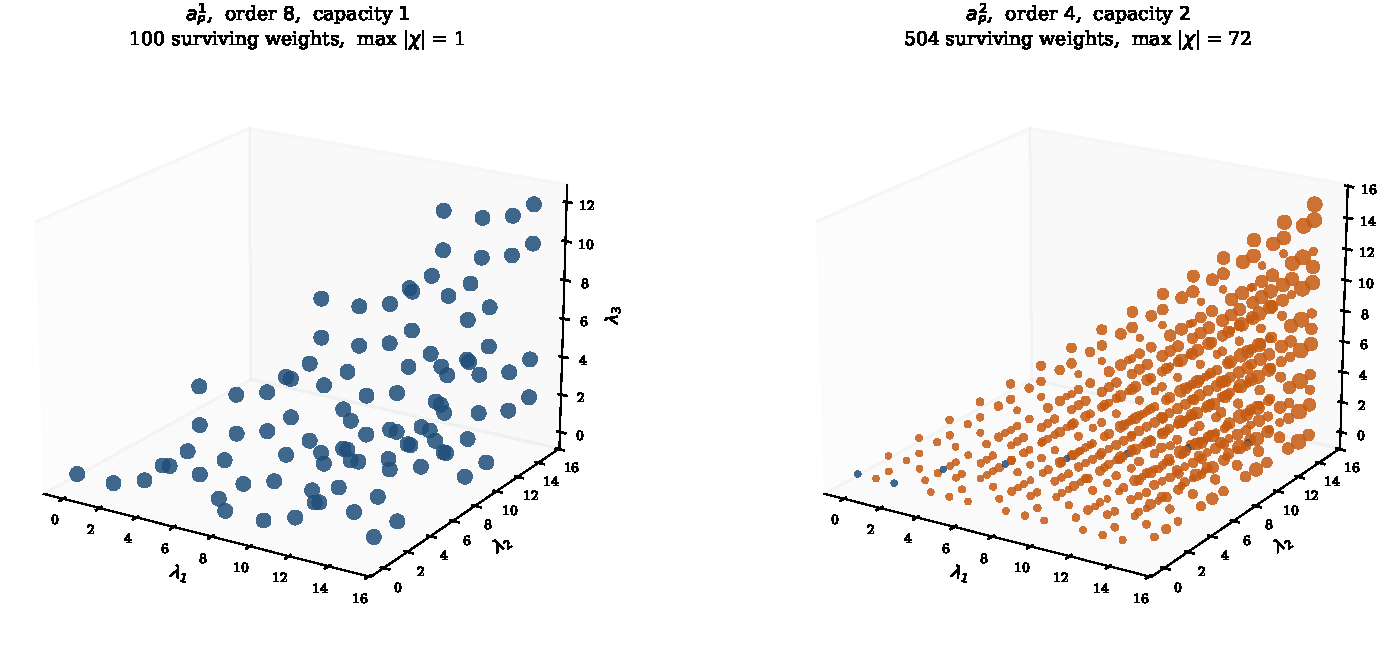
\includegraphics[width=\textwidth]{fig_union3d.pdf}
\caption{Por qué el contenido está en las potencias y no en $a_P$ mismo. Izquierda: capacidad uno,
$100$ supervivientes, todos los valores $\pm1$. Derecha: capacidad dos, $504$ supervivientes, con
valores hasta $72$. Las dos en $\Sp(6)$ sobre la caja $0\le\lambda_3\le\lambda_2\le\lambda_1\le15$. El tamaño del punto es $|\chi|$ y el azul marca $|\chi|=1$, así que los puntos
azules de la derecha son los que se comportan como si siguieran en $a_P$. En $a_P$ todo bloque del
centralizador es un toro y toda dimensión vale $1$ --- que es exactamente el caso $m=1$ de \cite{Prasad16b}.}
\label{fig:union3d}
\end{figure}



\begin{keybox}
\textbf{Y en tipo $C$ el lema está demostrado, así que el Teorema~\ref{thm:signo} se sostiene solo.}
El argumento de la Proposición~\ref{prop:Ms} se generaliza de $d=2$ a toda multiplicidad, con una
definición añadida: para un multiconjunto $U$ con repeticiones la parte de Vandermonde tiene que ser
el producto \emph{reducido} $A_{\mathrm{red}}(U)=\prod_{i<j,\ x_i\neq x_j}|1-x_i/x_j|$, ya que
$s\cdot\mu_q$ repite cada raíz $s$ veces y el producto sin reducir vale cero si $s>1$. Con
$A_{\mathrm{red}}$ en lugar de $A$ en todas partes, el argumento del borrado pasa igual. Con $d$
impar las capacidades quedan saturadas, las ocupaciones de todas las clases plegadas son las de
$\rho$, y cambios de signo y permutaciones de las coordenadas llevan un conjunto de residuos sobre el
otro. Con $d=2s$ queda una plaza libre, y el multiconjunto de las $m$ cantidades
$\xi_q^{(w\ell)_i}$ se escribe $U_a=s\cdot\mu_q-\{a\}$ con $a\in\mu_q$, siendo el de $\rho$ el
$U_1$. Escribiendo $M(U)$ para el producto reducido, $M(U)^2=A(U)^2C(U)D(U)$ en la notación de la
demostración de arriba, y borrar una copia de $a$ de $\mathcal B=s\cdot\mu_q$ da, por
$\prod_{y\in\mu_q,\,y\neq a^{-1}}|1-ay|=q$,
\[
A(U_a)=\frac{A(\mathcal B)}{q^{s}},\qquad
C(U_a)=\frac{C(\mathcal B)}{q^{2s}}F(a),\qquad
D(U_a)=\frac{D(\mathcal B)}{F(a)},
\]
con $F(a)=|1-a^2|$ si $a^2\neq1$ y $F(a)=1$ en otro caso, de modo que
$M(U_a)^2=A(\mathcal B)^2C(\mathcal B)D(\mathcal B)/q^{4s}$, independiente de $a$. Que los exponentes
que se anulan en el denominador recorran $q,2q,\dots$ en vez de valer todos $q$ no es un obstáculo:
quedan recogidos en $Z_q(\rho)$.
\end{keybox}

\subsection*{Qué es la diferencia de dos histogramas de residuos}

\noindent La Proposición~\ref{prop:res} dice que $\mathscr{R}_{\lambda+\rho}=\mathscr{R}_\rho$
cuando las capacidades del Corolario~\ref{conj:cap} se cumplen con igualdad. Cuando no, la
diferencia no es ruido: es el histograma de residuos de \emph{otro sistema de raíces}, de rango
acotado.

\begin{proposition}[la diferencia es la de otro grupo]\label{prop:resid}
Sea $\ell=\lambda+\rho$ con $N_q(\ell)=N_q(\rho)$, escríbase $m=uq+v$ con $0\le v<q$ y
$a=\lfloor(q-1)/2\rfloor$, y sea $S=\{s_1>\dots>s_r\}$ el conjunto de clases plegadas en que la
ocupación se aparta del perfil llano: las que llevan una fila de más cuando $v\le a$, con $r=v$;
las que llevan una de menos cuando $v>a$, con $r=q-v$. Con $T_q=\sum_{k=0}^{q-1}X^k$ y
$C_S=\sum_{c\in S}(X^c+X^{-c})$,
\[
P_\ell=\begin{cases}2u\,T_q+C_S, & v\le a,\\[1mm] 2(u+1)\,T_q-C_S, & v>a,\end{cases}
\]
y, con $H=C_r$ si $v\le a$ y $H=D_r$ si $v>a$, siendo $\rho_H$ su semisuma y
$\eta_i=s_i-(\rho_H)_i$,
\[
\boxed{\;\mathscr{R}_{\lambda+\rho}-\mathscr{R}_{\rho}
\;=\;\mathscr{R}^{H}_{\eta+\rho_H}-\mathscr{R}^{H}_{\rho_H}\;}
\]
\end{proposition}

\begin{proof}
Las dos formas de $P_\ell$ son los perfiles mínimos de la demostración del
Teorema~\ref{thm:cuenta}, que está enunciado para todo $q$: por debajo de
la mitad el perfil llano es $2u$ en cada clase no fija y $u$ en cada fija, y $v$ clases llevan una
fila más; por encima el perfil llano es uno más alto y $q-v$ clases llevan una menos. En
$\mathbb{Z}[X]/(X^q-1)$ se tiene $T_q^2=q\,T_q$ y $T_qC_S=2|S|\,T_q$. Como $\rho$ tiene el mismo
$u$ y $|S_0|=|S|$, todo término con $T_q$ es el mismo para $\ell$ y para $\rho$ y desaparece de la
diferencia; queda
\[
\mathscr{R}_{\lambda+\rho}-\mathscr{R}_\rho
=\frac{\bigl(C_S^2\pm C_S(X^2)\bigr)-\bigl(C_{S_0}^2\pm C_{S_0}(X^2)\bigr)}{2},
\]
con el signo que $C_S$ trae en $P_\ell$: elevar al cuadrado no lo ve, $X\mapsto X^2$ sí. Leída
\eqref{eq:res} en rango $r$, el signo de arriba es $\mathscr{R}^{C_r}$ y el de abajo
$\mathscr{R}^{D_r}$, porque $P(X^2)$ son exactamente las raíces largas $2e_i$ y $D_r$ no tiene
ninguna. Por último $S_0$ --- el conjunto de apartamiento del propio $\rho$ --- es $\rho_H$, luego
$C_{S_0}=P_{\rho_H}$ y $C_S=P_{\eta+\rho_H}$.
\end{proof}

\noindent \emph{Comprobado en $\mathbf{3\,729}$ pesos supervivientes con $m\le7$ y $q\le14$: la
identidad se cumple sin excepción, y también la forma intermedia de $P_\ell$ en los mismos
$3\,729$; la asignación de tipo no se cruza nunca, con $v\le a$ dando $C_r$ en $1\,365$ y $v>a$
dando $D_r$ en $2\,364$. Tres señuelos --- cambiar el tipo, desplazar $\eta$ en uno y no restar
$\rho_H$ --- rompen $447$, $407$ y $717$ de $1\,103$.}
\ver{residual\_histogramas.py}

\begin{keybox}
\textbf{Y eso es el corrector, medido.} Escríbase $\mathcal D(\lambda,q)$ para el producto de
dimensiones de la \S\ref{sec:dims} y $\kappa_q(\lambda)$ para la constante de allí. \emph{Sobre
$\mathbf{1\,814}$ pesos supervivientes con $m\le6$ y $q\le12$ --- todo $q$, no sólo los que
dividen a $t$ ---}
\[
\bigl|\chi_\lambda(g_{1/q})\bigr|
=\kappa_q(\lambda)\,\mathcal D(\lambda,q)\,\chi^{H}_{\eta}\bigl(h^{H}_{1/q}\bigr),
\]
\emph{sin excepción, donde $h^H_{1/q}$ es el punto de la recta de $\rho_H$ en $H$ con el mismo
denominador.} El punto residual es regular --- todo valor de raíz de $H$ queda estrictamente entre
$0$ y $q$ ---, así que nada se ha trasladado a un segundo límite singular. \emph{Cuatro señuelos la
rompen: desplazar $\eta$, cambiar el tipo, forzar $\kappa=1$ y tomar el residual igual a $1$ ---
que es el enunciado anterior --- fallan $390$, $386$, $371$ y $355$ de $1\,145$.} Fuera de las
cuatro familias el residual es donde va la irracionalidad: el factor entero se separa igual.
\emph{Esto es una medida, no un teorema: lo demostrado arriba es la identidad de histogramas, y el
paso de ella al valor absoluto y al signo no lo está.}
\ver{residual\_factorizacion.py}
\end{keybox}

\section{Una factorización en dimensiones}\label{sec:dims}

\noindent\emph{El valor salió como cociente de dos productos de enteros, y el cociente es siempre entero. ¿Está contando algo?}

El cociente $Z_q(\ell)/Z_q(\rho)$ se puede leer como un producto de dimensiones, una por clase
plegada. Antes de hacerlo, la literatura previa tiene que quedar en su sitio.

\begin{keybox}
\textbf{Factorizar un carácter clásico torcido en caracteres de grupos clásicos menores, indexados
por el $t$-cociente, es de Ayyer--Kumari.} Su Teorema~2.11 de \cite{AK22} hace exactamente eso para
$\mathrm{sp}_\lambda(X,\omega_tX,\dots,\omega_t^{t-1}X)$ --- el alfabeto \emph{sin borrar} --- y las
particiones que indexan los factores son las componentes de $\mathrm{quo}_t(\lambda)$, con $Sp$ y
$SO$ apareciendo como aquí. Lo que se hace abajo es la misma forma para el alfabeto de la
Proposición~\ref{prop:alph}, que es aquél \emph{menos dos letras}, especializado en $x_i=1$ para que
los caracteres se vuelvan dimensiones. Las dos letras borradas \emph{no} producen las clases fijas
--- ésas son las soluciones de $2c\equiv0\pmod q$, y existen por el plegado solo, una si $q$ es impar
y dos si es par --- pero sí cambian las \emph{ocupaciones} de esas clases, y con ellas el factor
$\kappa$. El patrón es suyo; el borrado, la especialización y $\kappa$ es lo que se
añade.
\end{keybox}

Sea $\lambda$ que cumple las capacidades. Para una clase no fija $c$ con $n$ filas, oriéntese cada
fila con un signo de modo que $\varepsilon_i\ell_i\equiv c\pmod q$, ordénense de mayor a menor los
enteros $y_i=(\varepsilon_i\ell_i-c)/q$, y póngase $\nu^{(c)}_i=y_i-y_n-(n-i)$. Para la clase fija
$0$ con filas $\ell_1>\dots>\ell_n$ póngase $\nu^{(0)}_i=\ell_i/q-(n-i+1)$; y si $q$ es par, para la
clase fija $q/2$, $\nu^{(q/2)}_i=\ell_i/q-(n-i+\tfrac12)$. Son particiones, y las clases vacías
aportan $1$.

\begin{theorem}[el módulo, factorizado]\label{thm:dims}
Con $D_c=\dim V^{GL_n}_{\nu^{(c)}}$ en una clase no fija, $D_0=\dim V^{Sp_{2n}}_{\nu^{(0)}}$ y
$D_{q/2}=\dim V^{SO_{2n+1}}_{\nu^{(q/2)}}$,
\[
\boxed{\;
\bigl|\chi_\lambda(a_P^{\,k})\bigr|\;=\;\kappa(\lambda)\,D_0\,D_{q/2}
\prod_{c\ \text{no fija}} D_c \;}
\]
omitiendo $D_{q/2}$ si $q$ es impar, donde $\kappa(\lambda)=1$ si $d$ es impar, $1$ si $d$ es par y
la plaza libre está en la clase $0$, y $2$ en otro caso.
\end{theorem}

\begin{keybox}
\textbf{Nada de la construcción usó $q\mid t$.} Las particiones $\nu^{(c)}$ se levantan de las
clases plegadas de $\ell$ y de las escaleras de las tres familias, y nada en esa receta sabe en qué
denominador está. Lo mismo vale para el cociente que calcula: \emph{sobre los $\mathbf{2\,186}$
pesos supervivientes de $\Sp(2m)$ con $m=2,\dots,5$ en todo $q=2,\dots,12$ --- y no sólo en los $q$
que dividen a $2m+2$ ---}
\[
\frac{Z_q(\lambda+\rho)}{Z_q(\rho)}\;=\;\kappa_q(\lambda)\,D(\lambda,q),
\qquad \kappa_q(\lambda)\in\{1,2\},
\]
\emph{sin excepción, con $\kappa_q=1$ en $1518$ de ellos y $2$ en $668$.} Lo que se demuestra abajo
es el caso $q\mid t$; el resto es medida, y dice que el teorema es más estrecho que su argumento. El
Teorema~\ref{thm:clasif} dice cuáles de esos denominadores son aquellos en los que el carácter mismo
es un número entero. \ver{teorema\_II.py}
\end{keybox}

\noindent La comprobación es sobre los denominadores de las fórmulas de dimensión. Tras salir las
potencias de $q$, las constantes de los bloques son $V_n=\prod_{j<n}j!$ para $GL_n$,
$C_n=2^n\prod_{j\le n}(2j-1)!$ para la clase $0$ y $B_n=\prod_{j\le n}(2j-1)!$ para la clase $q/2$;
con $d$ impar se cancelan contra el denominador, y con $d=2s$ mover la plaza libre fuera de la clase
$0$ produce exactamente el factor $2$, ya que $C_s/C_{s-1}=2(2s-1)!$ mientras
$V_{2s}/V_{2s-1}=B_s/B_{s-1}=(2s-1)!$. \emph{Medido sobre $\mathbf{11\,972}$ pesos supervivientes,
$m=2,\dots,7$, toda potencia: sin excepción.} \ver{dims\_recuento.py}

\noindent La plaza libre está determinada por $\lambda$ --- es la única clase cuya ocupación queda
una unidad por debajo de su capacidad ---, así que $\kappa$ está bien definida. \emph{Comprobado en
$10\,230$ pesos supervivientes con $d$ par: en todos hay exactamente una clase así.}
\ver{signo\_Fq.py}

\begin{keybox}
\textbf{Con $d$ impar el grupo no depende de $\lambda$ en absoluto.} Las capacidades quedan entonces
saturadas, así que todo peso superviviente tiene el \emph{mismo} perfil de ocupación --- y es el
perfil del propio $\rho$. \emph{Medido sobre $\mathbf{7\,166}$ pesos supervivientes con $d$ impar,
$m=2,\dots,9$: ni uno tiene otro perfil.} \ver{simplificaciones.py} Con lo cual, para $d$ impar el
producto $\prod_c D_c$ es una dimensión de un grupo fijo, el mismo para todo $\lambda$, y $\lambda$
sólo elige el peso máximo dentro de él: el Teorema~\ref{thm:dims} es una descomposición indexada por
bloques y no una coincidencia numérica. Con $d$ par exactamente un bloque pierde una fila, y
$\kappa$ registra cuál.

\smallskip
\textbf{Y el grupo lleva una huella.} Los bloques son $GL_{n}$ en las clases no fijas, $Sp_{2n}$ en
la clase $0$ --- y $SO_{2n+1}$ en la clase $q/2$. Ortogonal impar contra simpléctico es el par dual
de Langlands, y los dos recuentos de \cite{NPP25} se leen allí como dimensiones de centralizadores
en el grupo \emph{dual}. Es un indicio fuerte de a qué grupo pertenecen estas dimensiones, y es lo
que hace que la primera pregunta de la \S\ref{sec:preguntas} merezca la pena en vez de estar
meramente abierta.

\smallskip
\textbf{Y la huella es más vieja que el elemento.} Lecouvey \cite[\S3.2.2]{Lec07a} toma el alfabeto
\emph{completo}, pliega las clases de $\mu+\rho$ módulo $\ell$ igual que se pliegan aquí, y los tres
tipos ya están escritos en sus bloques: la clase $0$ lleva $\prod_{r\le s}(1-x_rx_s)$, que es tipo
$C$; los pares plegados llevan tipo $A$; y con $\ell$ par la clase $\ell/2$ lleva un Vandermonde de
tipo $B_{r_p}$, de semisuma $(\tfrac12,\dots,r_p-\tfrac12)$. Con $\ell$ impar lo cierra como
identidad --- un carácter del Levi $Sp\times GL\times\cdots\times GL$ \cite[Teor.~3.2.3]{Lec07a}.
\emph{Con $\ell$ par demuestra que no se puede:} esas raíces de tipo $B$ no están en el retículo de
raíces de $\Sp_{2n}$, y entonces los coeficientes \textbf{no son de ramificación y sus signos
alternan} \cite[Prop.~3.2.5]{Lec07a}.

\smallskip
\textbf{Qué es distinto aquí, y qué no.} Su Proposición~3.2.5 habla de los \emph{coeficientes} de
una descomposición, no de si un valor factoriza: en orden par y con el alfabeto completo el valor
sí factoriza, con su factor ortogonal impar, por el Teorema~2.11(2) de \cite{AK22}. Así que aquí
no se supera esa proposición, y el caso par no necesita rescate. Lo distinto es el alfabeto: es el
suyo menos dos letras (Proposición~\ref{prop:alph}), y el borrado es lo que mueve los perfiles y
pone la constante $\kappa\in\{1,2\}$ delante de las dimensiones.
\end{keybox}

\begin{keybox}
\textbf{Un ejemplo, que la receta tiene varios pasos.} En $\Sp(10)$ con $k=4$, o sea $d=4$, $q=3$ y
$p=1$, tómese $\lambda=(3,2,1,0,0)$. Entonces $\ell=(8,6,4,2,1)$, el cociente $Z_3(\ell)/Z_3(\rho)$
vale $8$ y $E_{1,3}(\lambda)=17$, luego $\chi_\lambda(a_P^4)=-8$; y la factorización dice
$\dim V^{GL_4}_{(1,1,1,0)}=4$ por $\dim V^{Sp_2}_{(1)}=2$.
\end{keybox}

\noindent Una advertencia que la forma invita a olvidar: son dimensiones de representaciones de
grupos construidos con los datos de \emph{cociente} de cada clase, no del centralizador de
$a_P^{\,k}$ mismo. Identificarlos con algo de ese lado pide un argumento que esta nota no tiene ---
véase la \S\ref{sec:preguntas}.

\section{Cuántos caracteres sobreviven}\label{sec:cuenta}

\noindent\emph{Ya sabemos qué pesos sobreviven y cuánto valen. ¿Cuántos son?}

El criterio es una condición sobre un punto y un arreglo de paredes módulo $q$, así que contar los
supervivientes es una pregunta sin teoría de representaciones dentro. Escríbase
$S_X(q)=\#\{x\in P/qP: N_q(x)=r_q\}$.


\begin{keybox}
\[
S_X(q)\;=\;\prod_{i=1}^{n}\,(q-m_i),\qquad m_i \text{ los exponentes de } W,
\]
\textbf{exactamente cuando} $r_q=0$ \textbf{y} $q$ es coprimo con los primos malos de $X$ ---
ninguno en tipo $A$, el $2$ en $B$, $C$ y $D$, y el $2$ y el $3$ en $G_2$, $F_4$ y $E_6$. Las cuatro
celdas de esa equivalencia, sobre los $298$ pares (tipo, $q$) medidos: $\mathbf{138}$ donde valen los
dos lados, $\mathbf{160}$ donde no vale ninguno, y \textbf{ninguno} en las dos celdas cruzadas. El
señuelo $\prod_i(q-i)$ --- que coincide con los exponentes en tipo $A$ y en ningún otro sitio ---
falla $221$ veces, así que el acuerdo es con los exponentes y no con el rango.
\ver{survivors\_law.py}
\end{keybox}

\noindent El miembro derecho es el producto de siempre; no reclamo nada nuevo sobre él, y esta nota
no lo necesita. Lo que compra la medida es la \emph{frontera}, y la frontera es donde vive el asunto
de esta nota. El orden de $a_P$ en $\Sp(2m)$ es $2m+2$, que es \emph{siempre par}, y el $2$ es un
primo malo en tipo $C$. Así que el recuento clásico no se aplica jamás en el segundo elemento de
Kostant, ni en ninguna de sus potencias --- y no por poco: en $q=6$ dentro de $C_2$, que es el propio
$a_P$, sobreviven ocho pesos donde el producto daría quince (Figura~\ref{fig:walls}).
\emph{Prueba:} en rango dos el caso par es visiblemente $S(q)=S(q-1)$ para
$B_2$ y $C_2$; sobrevive a rango tres en $C_3$ y \emph{se rompe en $B_3$}, donde $r_q=0$ y los
dos recuentos siguen difiriendo --- así que no es la regularidad de $\rho$ lo que lo gobierna.
Lo primero es encontrar qué lo sustituye. \emph{Qué compraría:} una
función generatriz en $q$ de cuánto del anillo de representaciones sobrevive en un elemento de
torsión, del lado de los dos elementos de Kostant donde ahora mismo no hay ninguna fórmula.
\ver{survivors\_quasipoly.py, survivors\_law.py}

\begin{figure}[tbp]
\centering
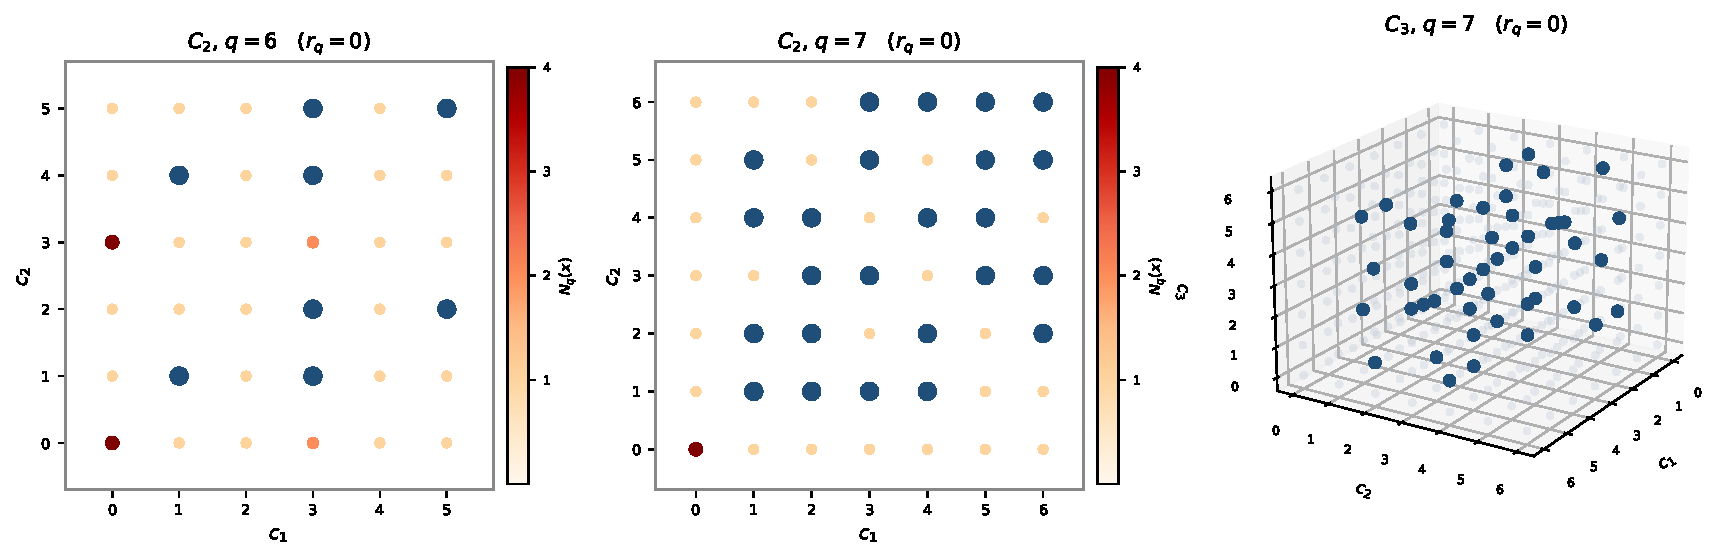
\includegraphics[width=\textwidth]{fig_walls.pdf}
\caption{El criterio es un punto esquivando paredes. Cada punto es un peso módulo $q$, en las
coordenadas $x=\sum_j c_j\omega_j$; azul quiere decir que ahí el carácter no se anula. El color de
los demás es $N_q(x)$, cuántas paredes toca el punto --- cuanto más oscuro, más divisibilidades
fuerza $\lambda$ por encima de las que $\rho$ ya forzaba. Izquierda, $C_2$ en $q=6$, que es el propio
$a_P$: $\mathbf{8}$ supervivientes donde $\prod_i(q-m_i)$ daría $15$. Centro, $C_2$ en $q=7$:
$\mathbf{24}$, y el producto da $24$. Derecha, el mismo dibujo una dimensión más arriba, $C_3$ en
$q=7$: $\mathbf{48}$, y el producto da $48$. La paridad de $q$, y nada más, separa los dos regímenes.
\ver{fig\_walls.py}}
\label{fig:walls}
\end{figure}


\noindent En tipo $C$ el recuento está cerrado para \emph{todo} $q$, y en un solo enunciado.
Escríbase
\[
f=\begin{cases}1,&q\text{ impar},\\2,&q\text{ par},\end{cases}
\qquad a=\frac{q-f}{2},
\qquad m=uq+v \ \ (0\le v<q).
\]

\begin{theorem}[el recuento, todo $q$, tipo $C$]\label{thm:cuenta}
\[
\boxed{\;
S_{C_m}(q)=
\begin{cases}
\dfrac{m!\;2^{\,2ua+v}\,\binom{a}{v}}
      {\bigl((2u+1)!\bigr)^{v}\,\bigl((2u)!\bigr)^{a-v}\,(u!)^{f}}, & v\le a,\\[6mm]
\dfrac{m!\;2^{\,a(2u+1)}\,\binom{a+f}{\,v-a\,}}
      {\bigl((2u+1)!\bigr)^{a}\,(u!)^{f}\,(u+1)^{\,v-a}}, & v>a.
\end{cases}\;}
\]
\end{theorem}

\noindent La demostración es el argumento de costes marginales de la \S\ref{sec:cap} al revés, y ése
nunca usó $q\mid 2m+2$: el coste de una fila más es $0,1,2,\dots$ en una clase no fija y
$1,3,5,\dots$ en una fija, así que el mínimo se alcanza llenando las plazas más baratas, y
$\rho=(m,\dots,1)$ lo alcanza --- sus residuos son $u$ vueltas completas de $\mathbb{Z}/q$ seguidas de
$1,\dots,v$. Cuando $v\le a$ cada clase fija lleva $u$ filas, $v$ clases no fijas llevan $2u+1$ y
las demás $2u$, que es lo que elige el binomio $\binom{a}{v}$; y cada fila de una clase no fija tiene
dos residuos posibles, que es la potencia de $2$. Cuando $v>a$ se parte de $2u+1$ en cada clase no
fija y $u$ en cada fija y se colocan las $b=v-a$ filas restantes en clases distintas; añadir una fila
multiplica el peso por $1/(u+1)$ tanto si la clase es fija como si no, luego las $\binom{a+f}{b}$
elecciones pesan igual. \emph{Comprobado contra enumeración exhaustiva en $40$ pares $(m,q)$: sin
discrepancias.} \ver{referee2.py}

\noindent \textbf{Las dos fórmulas del borrador anterior son los dos extremos de ésta.} Con $q>2m$
se tiene $u=0$ y $v=m\le a$, luego $S_{C_m}(q)=m!\,2^m\binom{a}{m}$, que es $\prod_i(q-(2i-1))$ si
$q$ es impar y $\prod_i(q-2i)$ si es par --- exponentes y grados, como arriba. Con $q\mid 2m+2$
devuelve el recuento multinomial sobre las capacidades, y en el propio $a_P$,
$S_{C_m}(2m+2)=2^m\,m!$. En el rango que quedaba abierto en medio da, por ejemplo,
$S_{C_3}(5)=72$ y $S_{C_3}(6)=96$.

\begin{keybox}
\textbf{Y una corrección que importa más que la fórmula.} Tienta llamar cuasipolinomio a $S_X(q)$ y
salir a buscarle el período. No lo es, globalmente. La literatura de cuasipolinomios característicos
cuenta el \emph{complemento} del arreglo modular --- los puntos que no están en ninguna pared ---,
mientras que $S_X(q)$ cuenta el estrato de nivel mínimo $r_q$, y $r_q$ cambia con $q$. Los dos
coinciden sólo donde $r_q=0$. Ya en $C_2$ se tiene $S_{C_2}(q)=(q-1)(q-3)$ para todo $q$ impar
grande, mientras que $S_{C_2}(3)=8$ y no $0$; y ningún período lo arregla, porque cualquier
progresión infinita de impares que contenga al $3$ fuerza el mismo polinomio. El enunciado correcto
es comportamiento cuasipolinómico \emph{eventual}, con un régimen singular aparte --- que es
exactamente lo que el Teorema~\ref{thm:cuenta} hace explícito.
\end{keybox}

\section{Una prueba fuera del tipo $C$: $G_2$}\label{sec:g2}

La regla de capacidades está escrita en las coordenadas del tipo $C$, así que la pregunta honesta
es qué sobrevive fuera de ellas. Quería dejarla abierta, y al escribir esto la probé en su lugar., y mientras escribía esto la medí. El
razonamiento era: una clase fija lleva $\lfloor d/2\rfloor$ porque el plegado es una involución, así
que en $G_2$, donde $r=3$, debería llevar $\lfloor d/3\rfloor$. Construí el evaluador que faltaba ---
multiplicidades de Freudenthal en $G_2$, contrastadas contra la fórmula de dimensiones de Weyl, y
devolviendo $\{0,\pm1\}$ en el propio $a_P$, que es el control que dice que el elemento es el bueno.

\begin{keybox}
\textbf{La predicción falló, y el enunciado bueno estaba al lado.} En $k=1$ el criterio ingenuo
transporta exacto --- $\chi_\lambda(a_P)=0$ ssi alguna raíz positiva cumple
$q\mid(\lambda+\rho,\alpha)$, $49$ de $49$. Donde el orden baja --- $d>1$, que entre $k=1,\dots,6$
significa $k=2,3,4,6$; en $k=5$ vuelve a ser $d=1$ y la regla ingenua sigue valiendo --- falla, y la
mejor de tres condiciones da $20$ de $49$. Pero es porque en una potencia el denominador ya lleva $r_q$ ceros forzados: preguntar si
\emph{alguna} raíz divide es la pregunta equivocada. Con \eqref{eq:crit} --- si hay \emph{más}
divisibilidades que las de $\rho$ --- $G_2$ cierra, y no como medida: \eqref{eq:crit} es un
enunciado sobre un sistema de raíces, así que se aplica aquí tal cual. Los valores, entretanto,
salen de $\{0,\pm1\}$ con holgura: con $k=4$ llegan a $343$.
\end{keybox}

\noindent En coordenadas: con $\lambda=a\omega_1+b\omega_2$, $u=a+1$ y $v=3(b+1)$, los seis valores
$(\lambda+\rho,\alpha)$ son $u,\;v,\;u+v,\;2u+v,\;3u+v,\;3u+2v$. Luego $N_q(\lambda)$ cuenta cuántos
de esos seis son divisibles por $q$, y $r_q$ es la misma cuenta sobre $1,3,4,5,6,9$. Aquí $t=12$ y
$q=12/\gcd(k,12)$, y dos valores de $q$ colapsan --- para \emph{todo} peso dominante, no para los
que me tocó correr:

\begin{corollary}\label{cor:g2}
En $G_2$: con $q=3$ (esto es, $k=4,8$), $\chi_\lambda(a_P^k)=0$ si y sólo si $a\equiv2\ (3)$; y con
$q=2$ (esto es, $k=6$), $\chi_\lambda(a_P^k)=0$ si y sólo si $a\equiv b\equiv1\ (2)$.
\end{corollary}

\begin{proof}
Con $q=3$, $v=3(b+1)\equiv0$, así que los seis valores se reducen a $u,0,u,2u,0,0$ y
$N_3=3+3\cdot[\,3\mid u\,]$, mientras que $r_3=3$, los múltiplos de $3$ entre $1,3,4,5,6,9$. Luego
$N_3=r_3$ exactamente cuando $3\nmid u=a+1$. Con $q=2$, $3u+v\equiv u+v$, $2u+v\equiv v$ y
$3u+2v\equiv u$, así que los seis se reducen a $u,\,v,\,u+v$ repetidos y
$N_2=2\,\#\{u,v,u+v \text{ pares}\}$; entre tres números de los que uno es la suma de los otros dos,
o hay exactamente uno par o lo son los tres, luego $N_2$ vale $2=r_2$ salvo que $u$ y $v$ sean ambos
pares, en cuyo caso vale $6$. Luego $N_2=r_2$ falla exactamente cuando $a$ y $b$ son ambos impares.
\end{proof}

\noindent \emph{Las dos congruencias comprobadas sobre los $\mathbf{40\,401}$ pesos con $a,b\le200$,
contra tres congruencias alteradas como señuelo, que fallan las tres.}
\ver{revision\_50\_G2\_corolario.py} \emph{Y el criterio mismo contra caracteres exactos de
Freudenthal --- que es el control de que el criterio es el bueno, no la prueba --- $49$ de $49$
pesos dominantes en cada $k=1,\dots,6$, sobre $0\le a,b\le6$.} \ver{revision\_47\_G2.py}

\noindent Eso no dice que $G_2$ no tenga teoría, sino que mi predicción estaba mal planteada.
«Clase fija» presupone las coordenadas $e_i$ y la involución sobre residuos que el tipo $C$ tiene;
$G_2$ no tiene ni una cosa ni otra, así que $\lfloor d/r\rfloor$ era una conjetura vestida de
consecuencia. La imagen de las capacidades parece un hecho sobre las \emph{coordenadas} del tipo
$C$, no sobre la razón de longitudes. Lo que hace en general el papel de una clase no es otro juego
de cubetas, sino la aplicación
\[
c_q(\lambda):Q\longrightarrow\mathbb{Z}/q,\qquad \alpha\longmapsto(\lambda+\rho,\alpha)\bmod q,
\]
tomada salvo $W$ --- un elemento de $\operatorname{Hom}(Q,\mathbb{Z}/q)/W$. En $C_m$, escrita sobre
$e_i-e_j,\ e_i+e_j,\ 2e_i$, ese dato se descompone justo en las cubetas plegadas $x\sim-x$. En $G_2$
es el punto $(u,v)$ y su incidencia con las seis paredes de raíz $u=0$, $v=0$, $u+v=0$, $2u+v=0$,
$3u+v=0$, $3u+2v=0$ módulo $q$; y $N_q(\lambda)$ cuenta a cuántas pertenece. Así que la noción
general es un punto de rango dos y un arreglo, no una cubeta unidimensional.
\ver{G2\_caracteres.py}

También intenté derivar el criterio de $G_2$ y me salió mal, de una manera que merece quedar
escrita: argumenté que si una reflexión deja fijo el exponente módulo $q$, sus dos términos se
cancelan. Se cancelan --- pero son dos términos de $|W|$. Lo cierto es que el numerador de Weyl se
anula siempre que el estabilizador del elemento contenga una reflexión, es decir \emph{siempre que el
elemento no es regular}, que es todo caso con $d>1$. Así que allí el numerador no dice nada y uno
vuelve al límite --- el mismo de la \S\ref{sec:cierre}.



\begin{keybox}
\textbf{Y en $q=3$ el valor mismo se cierra, signo incluido.} Con $\lambda=a\omega_1+b\omega_2$,
$u=a+1$ y $v=3(b+1)$, los exponentes divisibles por $3$ en un peso superviviente son $v$, $3u+v$ y
$3u+2v$, contra $3,6,9$ para $\rho$; los otros tres factores tienen igual módulo en los dos lados, y
los pisos de la \S\ref{sec:valor} dan el signo. Por tanto, para $k=4$ y $k=8$,
\[
\chi_{a\omega_1+b\omega_2}(a_P^{\,k})=
\begin{cases}
\ \ \dfrac{(b+1)(a+b+2)(a+2b+3)}{6}, & a\equiv0 \ (3),\\[3mm]
-\dfrac{(b+1)(a+b+2)(a+2b+3)}{6}, & a\equiv1 \ (3),\\[3mm]
\ \ 0, & a\equiv2 \ (3).
\end{cases}
\]
En $a=b=6$ eso da $7\cdot14\cdot21/6=343$, que es el valor que reporta la medida de arriba --- ahora
para toda la familia y no para la muestra.
\end{keybox}


\section{Una pieza de \cite{NPP25} con un solo peso cambiado}\label{sec:types}

\noindent Todo lo anterior cuenta raíces: el criterio, las capacidades, el valor, los
supervivientes. ¿Cuáles exactamente --- y es el conjunto que forman uno que la literatura ya
tenga clasificado? Lo es, con un solo peso cambiado.

El $R(m)$ de \cite{NPP25} selecciona raíces por altura, $\langle\beta,\rhoh\rangle$. La normalización de Kostant hace
que $\langle\alpha,x_P\rangle$ sea proporcional a $(\alpha,\alpha)$, así que para $a_P$ el estadístico
correcto da peso $1$ a las raíces simples cortas y $r$ a las largas. La llamo $P$-altura. Entonces
\[
\hgt_P(\alpha) \;=\; \tfrac{(\alpha,\alpha)}{2}\,\hgt(\alpha^\vee) \;=\; (\rho,\alpha),
\]
y la segunda igualdad es inmediata a partir de $\alpha^\vee=2\alpha/(\alpha,\alpha)$ y
$\langle\rho,\alpha_i^\vee\rangle=1$. Así que la $P$-altura \emph{es} el estadístico de raíces de
\eqref{eq:ps}, y el conjunto $R_P(q)$ de la \S\ref{sec:crit} --- cuyo tamaño daba $r_q$ --- es el de
las raíces de $P$-altura divisible por $q$. Ésa es la única razón de que esta sección pertenezca a
esta nota. \emph{Las dos lecturas comprobadas en todas las raíces positivas de
$B_3,B_4,C_3,C_4,C_5,F_4,G_2$ y todo $q\le24$, con la co-altura sola como señuelo, que difiere.}
\ver{revision\_52\_bisagra.py} Y:

\begin{observation}\label{obs:types}
Leído por corraíces, $R_P(q)$ siempre contiene al $R(q)$ calculado en el grupo dual; lo que tiene de
más son exactamente las raíces largas $\alpha$ de $G$ con $q \mid r\,\hgt(\alpha^\vee)$ pero
$q\nmid\hgt(\alpha^\vee)$; y los dos coinciden siempre que $\gcd(q,r)=1$.
\end{observation}

\begin{proof}
Bajo $\alpha\leftrightarrow\alpha^\vee$ la identidad de arriba dice
$\hgt_P(\alpha)=\hgt(\alpha^\vee)$ si $\alpha$ es corta y $\hgt_P(\alpha)=r\,\hgt(\alpha^\vee)$ si
es larga. Luego $q\mid\hgt(\alpha^\vee)$ implica $q\mid\hgt_P(\alpha)$ en los dos casos, que es la
contención; el recíproco sólo falla para una $\alpha$ larga con $q\mid r\,\hgt(\alpha^\vee)$ y
$q\nmid\hgt(\alpha^\vee)$, que es la parte extra enunciada; y si $\gcd(q,r)=1$ entonces
$q\mid r\,\hgt(\alpha^\vee)$ obliga a $q\mid\hgt(\alpha^\vee)$, luego no hay parte extra.
\end{proof}

\noindent Son tres líneas, así que la medida de abajo es un control y no la evidencia:

La Figura~\ref{fig:types} dibuja dónde se separan las dos selecciones.
$\mathbf{186}$ pares (tipo, $q$) en $B_n$, $C_n$ hasta $n=5$, $F_4$ y $G_2$, cada uno con
$2\le q\le 2h+1$, las tres
afirmaciones sin excepción. \ver{R\_P\_todos\_los\_tipos.py}

\noindent \textbf{Lo que eso no da.} Cuando $\gcd(q,r)=1$ las dos selecciones coinciden y la
clasificación de \cite{Polo25} --- que es una clasificación de los subsistemas cortados por
divisibilidad de la altura \emph{ordinaria} --- se traslada al lado de $a_P$ directamente. Cuando
$\gcd(q,r)>1$ no: las raíces largas de más pueden cambiar el tipo del subsistema, y en $G_2$ con
$q=3$ lo cambian. Allí $R_P(3)$ contiene las tres raíces largas positivas y es de tipo $A_2$,
mientras que la selección por coaltura divisible por $3$, antes de añadir las raíces extra, tiene una
sola raíz positiva. La observación se sostiene; la consecuencia clasificatoria necesita un argumento
que esta nota no da.

\begin{figure}[tbp]
\centering
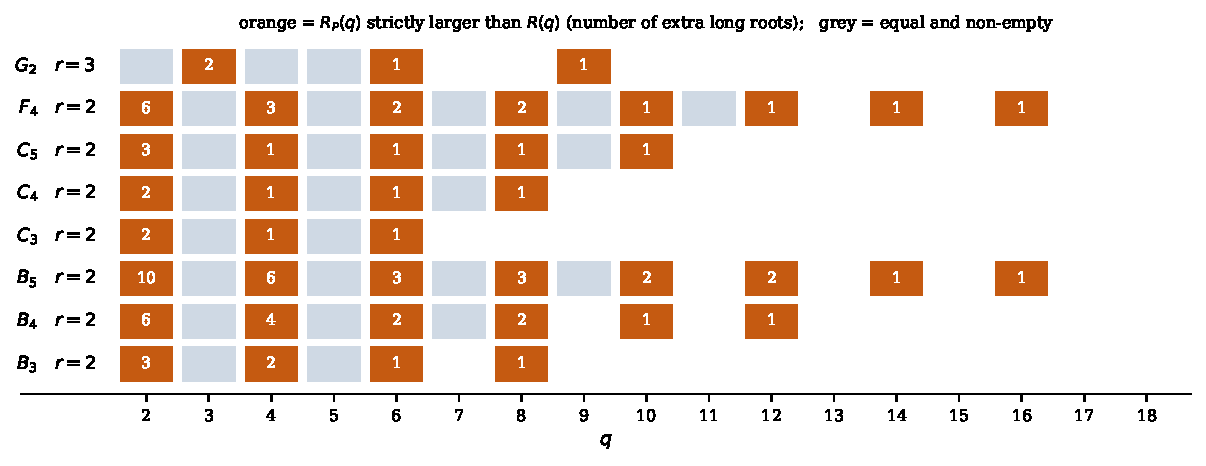
\includegraphics[width=\textwidth]{fig_types.pdf}
\caption{$B$, $C$ y $F_4$ se separan sólo en $q$ par; $G_2$ sólo en $q=3,6,9$, los múltiplos de su
$r=3$. El número de cada celda naranja es cuántas raíces largas de más lleva $R_P(q)$.}
\label{fig:types}
\end{figure}

\noindent El recíproco de la última cláusula es falso por un motivo tonto: para $q$ grande los dos
conjuntos están vacíos. Lo menciono porque mi primera versión era un «si y sólo si» con $32$
contraejemplos, $26$ de ellos exactamente ése y los otros $6$ una matriz de Cartan de $G_2$
transpuesta de mi lado.


\section{Lo que esto no es}\label{sec:open}

\begin{itemize}\itemsep2pt
\item \textbf{La máquina no es mía.} La ecuación \eqref{eq:ps} es la especialización principal
clásica; lo único que hice fue leerla en la recta de $\rho$, que es donde vive el segundo elemento de
Kostant. Lo que se añade aquí es el conteo de ceros \eqref{eq:crit}, la clasificación de los
denominadores en los que los valores son enteros (Teorema~\ref{thm:clasif}), y la combinatoria
que convierte el conteo en capacidades.
\item \textbf{Lo abierto está fuera del tipo $C$.} El Corolario~\ref{conj:cap} cierra la anulación
en tipo $C$, y el Teorema~\ref{thm:crit} la cierra en cualquier tipo. Dentro del tipo $C$ el valor
está completo: el Teorema~\ref{thm:valgen} da el valor absoluto para todo $k$, el Lema~\ref{lem:unit}
al que está condicionado es la Proposición~\ref{prop:Ms} en $d=2$ y la Proposición~\ref{prop:res} en
todo $d$, y el Teorema~\ref{thm:signo} da el signo. Lo que \emph{no} está demostrado es el
Lema~\ref{lem:unit} fuera del tipo $C$, donde \eqref{eq:res} todavía no tiene análogo. Y el signo,
aun determinado, no se simplifica: la \S\ref{sec:cierre} deja escrito dónde se ha buscado una forma
más corta y no está.
\item \textbf{El criterio no depende del tipo; las capacidades sí son de tipo $C$.} El conteo de
ceros \eqref{eq:crit} es un enunciado sobre un sistema de raíces y vale en cualquier tipo: en $C_m$
se vuelve el teorema de capacidades, y en $G_2$ el criterio de las seis paredes de la \S\ref{sec:g2}. La Observación~\ref{obs:types} habla también de sistemas de raíces, no de caracteres.
Caracteres puedo calcularlos en $C_m$ y en $G_2$, pero no en tipo $B$, donde haría falta el de
$\SO(2m+1)$.
\item \textbf{No se reclama ningún transporte de \cite{Prasad16}.} La demostración del
Teorema~\ref{thm:crit} es autocontenida y no usa ningún resultado de \cite{Prasad16}; si el argumento
de ese artículo alcanza también este criterio es una pregunta que esta nota no aborda.
\item Del artículo \cite{Polo25} he leído la introducción, la \S2 y lo bastante de la \S3.3 para confirmar
que la selección es por altura en todos los casos; las demostraciones caso por caso no las he leído.
\end{itemize}


\section{Lo que esto deja}\label{sec:preguntas}

En la familia $q\mid t$ el valor, su signo y el recuento quedan resueltos arriba, y el único paso
que era una medida --- la trivialidad del factor que no se anula --- es ahora la
Proposición~\ref{prop:res}. Pero el Teorema~\ref{thm:clasif} ha ensanchado el suelo bajo todo
eso: hay tres familias más en las que todo carácter es un número entero y en las que esta nota no
evalúa nada. Lo que sigue son las preguntas que quedan, de las cuales la primera no existía antes
de la \S\ref{sec:clasif}, y dos de las otras son más afiladas de lo que parecen porque la
respuesta obvia tiene contraejemplo.

\begin{enumerate}\itemsep5pt

\item \textbf{¿Cuánto vale en las otras tres familias?}
El Teorema~\ref{thm:clasif} lista cuatro familias de denominadores en los que todo carácter es
entero, y la \S\ref{sec:valor} evalúa una. En las otras tres la construcción de la
\S\ref{sec:dims} sigue funcionando --- la ficha de allí da $Z_q(\ell)/Z_q(\rho)=\kappa_q\,D$ en
todo $q$ medido --- pero el carácter no es $\pm\kappa_q D$: aparece un factor más, y su caso más
pequeño ya está en la \S\ref{sec:clasif}, donde $\Sp(4)$ con $q=4$ tiene
$Z_4(\ell)/Z_4(\rho)=1$ y $\chi_{(1,0)}=-2$. \emph{Qué es ese factor ya no está abierto.}
La Proposición~\ref{prop:resid} identifica la diferencia de los dos histogramas de residuos como
la de otro sistema de raíces, de rango a lo sumo $\lfloor q/2\rfloor$, y el recuadro que la sigue
lee el factor como el carácter de ese sistema en el mismo denominador --- sobre $\mathbf{1\,814}$
pesos supervivientes y en todo $q$, no sólo en los clasificados. En los puntos clasificados ese
carácter toma los valores $1,2,3,4$ y $6$, y nunca otro, sobre $\mathbf{828}$ pesos supervivientes
con $m\le5$ y $q\le12$. \emph{Lo que queda es el paso de la identidad al valor:} el tránsito del
histograma al valor absoluto y al signo, y la cancelación de las constantes de la \S\ref{sec:dims}
en todo $q$ y no sólo con $q\mid t$ --- esa cancelación está medida sobre $\mathbf{2\,186}$ pesos
supervivientes y demostrada sólo para $q\mid t$. \emph{Qué compraría:} el valor en todo el conjunto
clasificado y no en una cuarta parte de él, y también en los puntos sin clasificar.
\ver{teorema\_II.py, residual\_histogramas.py}

\item \textbf{¿De qué grupo son representaciones los $D_c$?}
El Teorema~\ref{thm:dims} escribe el módulo como producto de dimensiones de $GL_n$, $Sp_{2n}$ y
$SO_{2n+1}$, y con $d$ impar el perfil de bloques es el mismo para todo $\lambda$ superviviente
(\S\ref{sec:dims}). La conjetura natural --- un centralizador --- es \textbf{falsa por los dos
lados}. Tómese $m=6$, $k=7$, o sea $d=7$ y $q=2$: las dos clases fijas llevan tres filas cada una, el
grupo de la factorización es $Sp_6\times SO_7$, de tipo $C_3\times B_3$; pero $a_P^{\,7}$ tiene los
autovalores $1$ y $-1$ con multiplicidad seis cada uno, luego
$Z_{\Sp(12)}(a_P^{\,7})=Sp_6\times Sp_6$, de tipo $C_3\times C_3$. Y $C_3\times B_3$ tampoco puede
salir en el dual $SO(13)$: una descomposición en autoespacios allí produce factores lineales
generales y ortogonales, nunca un $C_3$ simple. \emph{Prueba:} buscar la construcción que mezcla un
factor simpléctico y uno ortogonal impar en las dos clases fijas --- que se distinguen porque
$2c\equiv0$ tiene las soluciones $0$ y $q/2$ --- sin suponer que sea el centralizador de nada.
\emph{Una construcción que sí los mezcla, y que merece probarse:} dentro de la superálgebra
$\mathfrak{osp}(1|2m)$, cuya parte par es $\mathfrak{sp}_{2m}$ y cuya parte impar es la
representación natural, tómese la subálgebra fija de $\mathrm{Ad}(-s_{\ell,q})$ y no la de
$\mathrm{Ad}(s_{\ell,q})$. En la parte par el signo no se ve y sale el centralizador de siempre;
en la impar ser fijo significa estar en el autoespacio de $-1$, así que sólo la clase $q/2$
conserva parte impar, y ésta se junta con su bloque simpléctico en
$\mathfrak{osp}(1|2n_{q/2})$. \emph{Comprobado por dimensiones en $\mathbf{1\,386}$ casos, con
$m\le7$ y $q\le12$: la subálgebra fija tiene exactamente las dimensiones de
$\bigoplus_c\mathfrak{gl}_{n_c}\oplus\mathfrak{sp}_{2n_0}\oplus\mathfrak{osp}(1|2n_{q/2})$, sin
excepción; con $m=6$ y $q=2$ es $\mathfrak{sp}_6\oplus\mathfrak{osp}(1|6)$, de dimensiones $42$ y
$6$.} \ver{osp.py} Que reaparezcan las dimensiones ortogonales impares es entonces la
correspondencia clásica entre $\mathfrak{osp}(1|2n)$ y las representaciones no espinoriales de
$\mathfrak{so}_{2n+1}$. \emph{Pero esto todavía no es una respuesta:} nada de aquí construye el
módulo a partir de $V_\lambda$, y la subálgebra depende del dato desplazado $\ell$, no del
elemento solo.
\emph{Qué compraría:} el Teorema~\ref{thm:dims} como regla de restricción y no como identidad de
números.
\emph{Y lo que se sabe del objeto vecino:} para el alfabeto completo --- la huella de la
\S\ref{sec:dims} --- Lecouvey demuestra que en el
rango estable $n>\max(\ell\,l(\lambda),l(\lambda'))$ los coeficientes del pletismo \emph{sí} son de
ramificación a un Levi, y los simplécticos pasan por $V^{\mathfrak{so}_{2n+1}}(\lambda')$
\cite[Teor.~4.5.1]{Lec07b}; mientras que con $\ell$ par y fuera de ese rango \emph{no} lo son y sus
signos alternan \cite[Prop.~3.2.5]{Lec07a}. Ninguna de las dos responde la pregunta de aquí --- el
objeto de abajo es un valor, y sobre un alfabeto más corto --- pero dicen dónde está el obstáculo,
y es otra vez el obstáculo de retículo de tipo $B$ de la \S\ref{sec:dims}.

\item \textbf{¿Qué le hacen al cociente las dos letras borradas?}
Para el alfabeto \emph{sin borrar} la respuesta es \cite{Lec07a} y \cite{AK22}, y el plegado en
clases ya es de Lecouvey, quince años antes: los factores están indexados por las
componentes de $\mathrm{quo}_t(\lambda)$. Aquí los $\nu^{(c)}$ de la \S\ref{sec:dims} están
construidos a mano, y lo natural es que sean las componentes de un $q$-cociente del alfabeto
borrado. La analogía hay que enunciarla con cuidado: en tipo $A$ el criterio clásico del núcleo es
sobre una especialización en un multiconjunto \emph{completo} de raíces $q$-ésimas y es falso para
una especialización principal cualquiera --- $s_{(1)}(1,-1,1)=1$ aunque $(1)$ tiene $2$-núcleo no
vacío. \emph{Prueba:} comparar $\nu^{(c)}$ con $\mathrm{quo}_q$ del beta-conjunto de $\lambda$ donde
los dos están definidos, y ver qué mueven los dos borrados. \emph{Qué compraría:} la
\S\ref{sec:dims} como corolario de \cite{AK22} y no como identidad paralela.

\item \textbf{Fuera del tipo $C$, la mitad abierta es el módulo, no el signo.}
La derivación por senos del Teorema~\ref{thm:signo} no usa el tipo: con la normalización de la
\S\ref{sec:norm} da el signo dondequiera que el criterio se aplique. Lo que se creía de tipo $C$ es
la Proposición~\ref{prop:res} --- y \eqref{eq:adj} dice que su primera mitad no lo es: vale en
todo tipo. Lo que \emph{no} se generaliza es la forma: $\mathrm{Sym}^2$ y $\Lambda^2$ de la
representación natural cubren los tipos clásicos y no dicen nada de los excepcionales, donde el
único enunciado es \eqref{eq:adj} misma. Su segunda mitad vale allí
donde $\ell$ cae en la órbita $\widehat W_q^{+}\!\cdot\rho$, otra vez en todo tipo. \emph{Así que lo
abierto de verdad es la plaza libre:} los supervivientes fuera de esa órbita, que aparecen
exactamente con $d$ par y $q\ge3$. \emph{Prueba:} cerrarlos en $B_m$ y en $F_4$, donde la razón de
longitudes vuelve a ser $2$ pero las coordenadas son otras. \emph{Y la medida dice que merece la
pena:} $\mathscr{R}_\ell=\mathscr{R}_\rho$ se comprobó en los $\mathbf{1\,463}$ pesos supervivientes
de $B_2,B_3,B_4$ y en los $\mathbf{861}$ de $G_2$ sobre los cinco $q\mid12$ --- sin excepción, en
tipos donde esta nota no demuestra nada. \ver{lema\_generico.py} \emph{Y un aviso que toda extensión tiene que respetar:} la forma cerrada
\textbf{no} vale en un punto cualquiera de la recta de $\rho$, ni siquiera en tipo $C$. En $\Sp(4)$
con $\lambda=(1,0)$ y $q=7$ ningún exponente es divisible por $7$, luego $Z_7(\ell)/Z_7(\rho)=1$,
mientras que $\chi_{(1,0)}(g_{1/7})=2\cos\frac{2\pi}{7}+2\cos\frac{4\pi}{7}=0.8019\ldots$ El
criterio vale en toda la recta; la fórmula del \emph{valor} es un enunciado sobre los puntos
clasificados del Teorema~\ref{thm:clasif}, y $q=7$ con $m=2$ no es uno de ellos.

\item \textbf{¿Cuál es el recuento fuera del tipo $C$?}
El Teorema~\ref{thm:cuenta} cierra $S_{C_m}(q)$ para todo $q$, y la \S\ref{sec:cuenta} deja escrito
que en el régimen regular la respuesta se lee por exponentes con $q$ impar y por grados con $q$ par.
Esa alternancia es exacta en $A$ y en $C$ y \emph{se rompe en $B_3$}, cuyo retículo de pesos lleva el
peso spin. \emph{Prueba:} rehacer el recuento por costes marginales en $B_m$ y $D_m$ con $P$ y no con
$\mathbb{Z}^m$, y ver si el índice del retículo entra como factor o cambia la forma. \emph{Qué compraría:}
un teorema de recuento para los tipos clásicos en vez de uno para $C$, y el principio de una
respuesta para los excepcionales.

\item \textbf{La recta de $\rho$ no contiene a $a_Q$: ¿qué familia contiene a los dos?}
Tienta leer la \S\ref{sec:crit} como si pusiera los dos elementos de Kostant en una misma recta, y
eso es falso. En $\Sp(4)$ el levantamiento de $a_Q$ que usa la \S\ref{sec:controles} tiene espectro
$\{\zeta_8,\zeta_8^3,\zeta_8^5,\zeta_8^7\}$, mientras que un punto de la recta de $\rho$ tiene
espectro $\{z,z^{-1},z^2,z^{-2}\}$; si $z$ fuera uno de esos autovalores tendría orden $8$, y
entonces $z^2$ tendría orden $4$ y no estaría en el espectro de $a_Q$. No sirve ningún $z$.
\emph{Prueba:} tomar la familia de dos parámetros
$\exp(2\pi i(\theta\rho^\sharp+\theta'\rho^{\vee\sharp}))$ y preguntar en qué puntos suyos sigue
cerrando el argumento de la \S\ref{sec:crit}. \emph{Qué compraría:} la unificación que la
\S\ref{sec:map} dibuja como dos líneas que se juntan en una caja, enunciada como matemáticas y no
como imagen.

\end{enumerate}

\appendix
\section{Lo que se intentó por el camino, y no salió}\label{sec:cierre}

\noindent \emph{Lo que sigue es un registro, no un resultado.} El Corolario~\ref{conj:cap} dice que
en $z=\xi_q$ los dos lados de \eqref{eq:ps} se anulan al mismo orden, luego el carácter es un límite
--- y un límite es un cálculo, no un programa. La \S\ref{sec:modulo} hace ese cálculo. Lo que se
conserva aquí es el camino recorrido antes de encontrarlo, porque quien tenga que decidir cuánto
fiarse del resultado debería poder ver cuáles de las vías evidentes se probaron y dónde se paró
cada una. Es decir:

\begin{keybox}
\textbf{Problema.} En $z=\xi_q$ el numerador y el denominador de \eqref{eq:ps} se anulan al mismo
orden --- eso es exactamente \eqref{eq:crit}, que es el Corolario~\ref{conj:cap} --- de modo que el
carácter es el límite
\[
\chi_\lambda(a_P^k)\;=\;\xi_q^{-(\lambda,\rho)}\lim_{z\to\xi_q}\ \prod_{\alpha>0}
\frac{1-z^{(\lambda+\rho,\alpha)}}{1-z^{(\rho,\alpha)}} .
\]
\textbf{Ese límite ya está evaluado.} Sacar factor común a
los $r_q$ factores que se anulan a cada lado da el cociente de los \emph{productos} de sus
exponentes --- no hay emparejamiento canónico raíz a raíz, ni hace falta. Eso es el
Teorema~\ref{thm:valgen}, y vale en todo $d$ siempre que los factores que sobreviven no aporten nada
al módulo, que es el Lema~\ref{lem:unit}: demostrado en $d=2$ por la Proposición~\ref{prop:Ms} y, en
tipo $C$, en todo $d$ por la Proposición~\ref{prop:res}. \textbf{Lo que queda de esta vía está fuera
del tipo $C$}, donde \eqref{eq:res} todavía no tiene análogo --- y allí el lema sigue siendo
aritmética finita, dos productos explícitos de $1-\xi_q^{\,r}$ con el mismo módulo, sin teoría de
representaciones a la vista.
\end{keybox}

\smallskip
\noindent\textbf{Dos cosas que el signo no es.} El Teorema~\ref{thm:signo} da el signo como una suma
de partes enteras, y la \S\ref{sec:valor} enseña que el candidato más limpio no sobrevive a la
comprobación. Lo que sigue es el resto de esa búsqueda, que merece quedar escrito porque dice hasta
qué punto el signo es un invariante fino. En $k=2$ el alfabeto da $H(z)=(1-z)^2/(1-z^q)^2$, así que el
carácter es un determinante entero y su signo es un dato duro, sin ningún juicio numérico dentro.
Sobre $\mathbf{4\,301}$ pesos supervivientes en $\Sp(2m)$ con $m=2,\dots,9$, el
Teorema~\ref{conj:val} se cumple sin una sola discrepancia --- lo que además extiende su verificación
a $m=7,8,9$. Sobre esa muestra:

\begin{itemize}\itemsep2pt
\item el signo \textbf{no es función del patrón de ocupación}. De los $32$ patrones de «qué clases
llevan $0$, $1$ o $2$ filas» que aparecen, \emph{ninguno} lleva signo constante. El testigo mínimo
está en $\Sp(4)$ con $k=2$: $\lambda=(1,0)$ y $\lambda=(1,1)$ ocupan las mismas clases y tienen
el mismo módulo $2$, y sus caracteres son $-2$ y $+2$. El signo lee los números, no la forma.
\item y \textbf{no es una combinación lineal sobre $\mathrm{GF}(2)$} de quince paridades naturales:
cuántas clases toman la rama $+$ de $\mp$ y cuántas la $-$, la paridad de los cocientes
$\lfloor\ell_i/q\rfloor$, la de las filas dobladas, la de $|\lambda|$, la de $(\lambda,\rho)$, la de
las inversiones de la palabra de clases, el índice de la clase libre, y otras. El sistema lineal
sobre los $2\,582$ pesos con $m\le6$ es \emph{incompatible} --- ningún subconjunto sirve, así que no
hubo que validar ninguno en los $1\,719$ pesos de $m=7,8,9$ que se habían apartado para eso. Una
columna de paridades aleatorias viajó dentro del ajuste como señuelo.
\end{itemize}

\noindent Es un resultado negativo, y es lo que hace que el segundo punto de abajo merezca el tiempo
de alguien y no una tarde: el signo es un invariante más fino que los candidatos naturales, y donde
más probablemente se esconde una forma más corta es en el mismo sitio del que salió el módulo --- el
elemento de Weyl que ordena los residuos, cuya longitud no es función de las clases solas.
\ver{sign\_k2.py}

\noindent La otra entrada es la diferencia finita de la \S\ref{sec:alph} --- la pregunta que quedó
allí planteada. Tiene respuesta, y la tuve al revés durante dos días, así que dejo las dos. Creía
que la obstrucción era que el desplazamiento actúa sobre $b_i+j$ y $b_i-j$ con signos opuestos y por
eso no factoriza. Sí
factoriza: el desplazamiento mueve el \emph{índice} de $h$, y $h_{b_i\pm j}\mapsto h_{(b_i-1)\pm j}$
es un desplazamiento de $b_i$ en \emph{los dos} sumandos; el signo de $j$ no interviene nunca. Por
multilinealidad en filas, para todo polinomio $P$,
\[
D_{P(S)h}(\mathbf b)=\Bigl(\prod_{i=1}^{m}P(T_i)\Bigr)D_h(\mathbf b),
\qquad (T_iF)(\dots,b_i,\dots)=F(\dots,b_i-1,\dots),
\]
y en particular $D_A=\prod_i(1-T_i)^2 D'$ para $d$ par y $\prod_i(1-T_i^2)D'$ para $d$ impar.
\emph{Comprobado numéricamente hasta $10^{-14}$, con señuelo que falla.}
\ver{revision\_47\_verificacion.py}

\noindent Así que la ramificación no es el obstáculo que yo hacía de ella, y la diferencia segunda
sí atraviesa el determinante. Lo que queda por esa vía es la cancelación entre determinantes con
beta-números desplazados --- y dentro del tipo $C$ ya no hace falta nada de eso, porque la anulación
la resuelve \eqref{eq:crit} y el valor la Proposición~\ref{prop:res}. Fuera de él yo empezaría por
el límite de la ficha de arriba, porque lleva los exponentes explícitos.

Hay un sitio donde miraría, y lo encontré tarde: el segundo artículo de Kumari
\cite{Kum24} trata $\Sp_{2tn+2}$ --- el alfabeto grande \emph{más} un par. Lo que esta nota necesita
es el alfabeto grande \emph{menos} un par. Es el caso contiguo, hecho con fórmulas de caracteres de
Weyl y beta-conjuntos de $t$-núcleos, y si esa maquinaria corre hacia atrás puede ser la respuesta
entera.

Y ahí es donde se para. Lo que más me gustaría saber, por orden:
\begin{itemize}\itemsep2pt
\item el \textbf{Lema~\ref{lem:unit} fuera del tipo $C$.} Dentro de él, la afirmación (B) de la
\S\ref{sec:modulo} demuestra el lema y con él todo el Teorema~\ref{thm:valgen}, y (B) es una
congruencia entre dos multiconjuntos de residuos sin un carácter dentro. Sobre lo que se apoya es
\eqref{eq:res}, escrita en las coordenadas del tipo $C$; esa misma congruencia en otro sitio es todo
lo que al valor le sigue faltando;
\item una \textbf{forma más corta del signo} que la suma de partes enteras --- y los dos negativos
de arriba dicen que no es ni función del patrón de ocupación ni una paridad de los estadísticos
naturales;
\item si el lema de filas más la cancelación entre determinantes desplazados llega por el otro
camino, y si el $\Sp_{2tn+2}$ de Kumari \cite{Kum24} corrido hacia atrás es esa cancelación.
\end{itemize}

\section{Los controles, en el orden en que se corrieron}\label{sec:controles}

Nada de lo que sigue hace falta para una demostración. Se conserva porque los enunciados de arriba se
midieron antes de derivarse, y quien decida cuánto fiarse de ellos debe poder ver qué se corrió.


\subsection*{Primero, el Teorema~2 de \cite{Prasad16b} --- recalculado, no citado}

En $t=1$ --- otra vez el elemento del toro de ese artículo, no el $2m+2$ de éste --- su alfabeto es
$\mu_n$ con multiplicidad $m$, luego
$H(z)=\prod_{\omega^n=1}(1-\omega z)^{-m}=(1-z^n)^{-m}$, los $h_k$ son enteros y el determinante es
exacto. Implementé el enunciado desde cero y lo corrí.

\begin{center}
\small
\rowcolors{2}{white}{filaclara}
\begin{tabular}{ccrccc}
\toprule
\rowcolor{cabecera}$m$ & $n$ & pesos & criterio & valor & señuelos (un bloque menos / más)\\
\midrule
1&3& 84 & $84/84$ & $84/84$ & $27$ / $27$\\
2&2& 210 & $210/210$ & $210/210$ & $40$ / $40$\\
2&3& 462 & $462/462$ & $462/462$ & $72$ / $54$\\
3&2& 462 & $462/462$ & $462/462$ & $60$ / $40$\\
2&4& 495 & $495/495$ & $495/495$ & $54$ / $54$\\
3&3& 220 & $220/220$ & $220/220$ & $32$ / $32$\\
4&2& 495 & $495/495$ & $495/495$ & $45$ / $45$\\
\midrule
\multicolumn{2}{c}{total} & $\mathbf{2428}$ & $100\%$ & $100\%$ & \\
\bottomrule
\end{tabular}
\end{center}

\noindent La última columna es el control: una fórmula con un bloque de menos, o uno de más, acierta
entre el $8{,}7\%$ y el $32{,}1\%$ de las veces. \ver{prasad2016\_vs\_nuestro.py}


\subsection*{Segundo, el otro elemento}

Con $\ell=\lambda+\rho$, $d=\gcd(k,t)$ y $q=t/d$:


\noindent Medí primero una regla sobre capacidades --- los $31$ pares $(m,k)$ con $m=2\ldots7$,
$k=1\ldots6$ y $q\ge3$, sobre $\lambda_1\le8$ (o $\le6$ si $m\ge5$): $\mathbf{21\,630}$ pesos
dominantes, sin excepción \ver{aP\_potencias.py} --- y después, una vez que la
Proposición~\ref{prop:alph} dijo que el elemento vive en la recta de $\rho$, resultó ser la sombra
en tipo $C$ de algo que no menciona el tipo $C$ en absoluto.

\smallskip

\subsection*{Tercero, el control: la misma prueba sobre el otro elemento de Kostant}

Una regla que encaja podría ser, aun así, una regla sobre escaleras y no sobre $a_P$. Así que corrí
la misma prueba con $a_Q$ dentro del mismo grupo. En $\Sp(2m)$ el elemento de Coxeter es la escalera
impar $(1,3,\dots,2m-1)$ a orden $4m$ --- $\rhoh$ es semientero, de modo que el levantamiento tiene
orden $2h$ --- y comprobé que empareja a $1$ con toda raíz simple, cosa que la escalera par no hace.

Después, para cada $(m,k)$, pregunté qué parejas (capacidad en clase no fija, capacidad en clase
fija) de entre todas las de $\{0,\dots,4\}^2$ reproducen exactamente la anulación.

\begin{keybox}
Para $a_P$ la respuesta es siempre $(d,\lfloor d/2\rfloor)$ y ninguna otra. \textbf{Para $a_Q$ no
suele haber respuesta}: en $14$ de los $16$ casos corridos, \emph{ninguna} pareja de capacidades
reproduce la anulación. Así que la regla no es un hecho sobre escaleras. Es un hecho sobre $a_P$, y
la Proposición~\ref{prop:alph} dice por qué: el alfabeto de $a_Q^{\,k}$ vive en los residuos
\emph{impares}, y no es $d\cdot\mu_q$ menos dos puntos en absoluto.
\end{keybox}

\noindent Es el control que más me habría gustado que alguien corriera contra mí, así que lo corrí
antes de enviar esto. \ver{aQ\_potencias.py}


\section*{Atribución}\label{tab:attrib}

{\small
\rowcolors{2}{white}{filaclara}
\begin{longtable}{@{}p{0.40\textwidth}p{0.55\textwidth}@{}}
\toprule
\rowcolor{cabecera}el alfabeto, como multiconjunto de $\mu_q$ & de quién es\\
\midrule
\endfirsthead
\toprule
\rowcolor{cabecera}el alfabeto, continuación & \\
\midrule
\endhead
$c\cdot\mu_q$ \emph{exacto} --- el alfabeto completo
 & Littlewood \cite{Li40}; Prasad \cite{Prasad16b}, Teor.~2, en $\GL$;
   Ayyer--Kumari \cite{AK22} en los grupos clásicos; Albion \cite{Alb23} en los caracteres
   universales; y Lecouvey \cite{Lec07a,Lec07b}, independientemente, por pletismos --- la
   atribución conjunta es del propio Albion \cite{Alb25}\\
$c\cdot\mu_q$ \emph{más} una tirada parcial de $m$ letras & Kumari \cite{Kum24}, Teor.~2.2\\
\textbf{los tres tipos en las clases plegadas --- $C$ en la clase $0$, $A$ en los pares plegados,
$B$ en la clase $q/2$ --- y que con $\ell$ par no son coeficientes de ramificación}
 & \textbf{Lecouvey \cite{Lec07a}}, \S3.2.2, Teor.~3.2.3 y Prop.~3.2.5, en el alfabeto
   \emph{completo}; en el rango estable, y por $V^{\mathfrak{so}_{2n+1}}(\lambda')$,
   \cite{Lec07b}, Teor.~4.5.1\\
$c\cdot\mu_q$ \emph{más} una letra $1$ & Kumari \cite{Kum24}, Teor.~2.8\\
con soporte en los residuos \emph{impares} --- que es el alfabeto de $a_Q$, no el de $a_P$
 & Ayyer--Kumari \cite{AK25}, \S3\\
cualquier alfabeto con $q=2$ --- los elementos de orden $2$ & Karmakar \cite{Kar24}, Teor.~5.1\\
\midrule
\rowcolor{marca}$c\cdot\mu_q-\{1\}-\{-1\}$ (Prop.~\ref{prop:alph}, $d$ impar) & esta nota\\
\rowcolor{marca}$c\cdot\mu_q-2\cdot\{1\}$ (Prop.~\ref{prop:alph}, $d$ par) & esta nota\\
\midrule
$c\cdot\mu_q-\{1\}$ --- una sola letra, en el punto fijo
 & \emph{sin fuente en la literatura comprobada aquí}\\
\bottomrule
\end{longtable}}

\vspace{4pt}
\noindent Ése es el eje, porque el alfabeto decide a la vez qué es verdad y de quién es. Todo
alfabeto del bloque de arriba es un múltiplo entero de $\mu_q$, o eso con una tirada corta
añadida; las dos filas de esta nota son ese múltiplo \emph{menos} a lo sumo dos letras, y esas
letras son los puntos fijos de $w\mapsto w^{-1}$. La fila sin fuente es una tercera de la misma
clase, que cubre el argumento de la \S\ref{sec:modulo} y que no se enuncia abajo.
\emph{Esto describe las familias listadas, no clasifica la recta de $\rho$: hay denominadores
fuera de todas ellas en los que el factor no nulo se cancela igual --- $\Sp(14)$ con $q=6$ es
uno, y su alfabeto no tiene esta forma en absoluto.} \ver{alfabeto\_clasif2.py}

\vspace{6pt}
{\small
\rowcolors{2}{white}{filaclara}
\begin{longtable}{@{}p{0.52\textwidth}p{0.43\textwidth}@{}}
\toprule
\rowcolor{cabecera}lo demás sobre lo que se apoya esta nota & \\
\midrule
\endfirsthead
\toprule
\rowcolor{cabecera}tabla de atribución, continuación & \\
\midrule
\endhead
$\{0,\pm1\}$ en $a_Q$ y en $a_P$; los dos elementos & Kostant \cite{Kostant76}\\
torcido $=$ plegado, y $A_{2m}\to C_m$ & Kumar--Lusztig--Prasad \cite{KLP09}\\
la sombra en los grupos de Weyl, $\Theta(w_0)=\pm\dim$ & Lübeck--Prasad \cite{LP20}\\
$R(m)$, $d_m$, y su clasificación & NPP \cite{NPP25}, Polo \cite{Polo25}\\
la regla de tipo $C$ como identidad & Pétréolle \cite{Petreolle15}, Wahiche \cite{Wahiche23}\\
la regla de tipo $A$ con núcleos & Adin--Frumkin \cite{AF02}\\
\midrule
la especialización principal \eqref{eq:ps} & clásica\\
\textbf{el criterio \emph{y} el signo en $a_P$ mismo, en todo tipo; su forma en tipo $C$; y el signo
leído en los residuos ordenados} & \textbf{Cellini--Möseneder Frajria--Papi \cite{CMP06}},
Cor.~3.2, Prop.~3.5 y Obs.~3.2\\
la forma en corraíces del criterio, para todo entero & NPP \cite{NPP25}, Cor.~3.7\\
\midrule
\rowcolor{white}\multicolumn{2}{l}{\emph{y lo que se hace aquí, aparte de las dos filas de alfabeto:}}\\
\textbf{qué denominadores de la recta de $\rho$ dan valores enteros} (Teor.~\ref{thm:clasif}) & \\
el mismo conteo en toda la recta de $\rho$, en las potencias (Teor.~\ref{thm:crit}) & \\
la combinatoria que lo vuelve capacidades (Cor.~\ref{conj:cap}) & \\
la unidad de holgura, y de dónde sale (Prop.~\ref{prop:slack}) & \\
el valor absoluto en $k=2$ (Teor.~\ref{conj:val}) & \\
el valor absoluto en todo $k$ (Teor.~\ref{thm:valgen}), salvo el Lema~\ref{lem:unit} & \\
el lema de residuos \eqref{eq:res}, y \eqref{eq:adj} detrás (Prop.~\ref{prop:res}) & \\
el valor exacto con su signo, \emph{toda} potencia, tipo $C$ (Teor.~\ref{thm:signo}) & \\
su módulo factorizado en dimensiones, con $q\ge3$ (Teor.~\ref{thm:dims}) & \\
el recuento cerrado de los supervivientes, todo $q$, tipo $C$ (Teor.~\ref{thm:cuenta}) & \\
el mismo criterio en $G_2$, y sus dos congruencias (Cor.~\ref{cor:g2}) & \\
que el signo no es ni una forma ni una paridad (\S\ref{sec:cierre}) & \\
el lema de filas para una sucesión $h$ desplazada (\S\ref{sec:cierre}) & \\
la $P$-altura, y la comparación de la Figura~\ref{fig:types} (Obs.~\ref{obs:types}) & \\
\bottomrule
\end{longtable}}

\vspace{3pt}
\noindent Los bloques superiores no son míos, y nada del inferior existiría sin ellos. Dos líneas
merecen leerse despacio. \textbf{En $a_P$ mismo --- $k=1$ --- el criterio y el signo son el
Corolario~3.2 de \cite{CMP06}}, en todo tipo y en el estadístico de \emph{raíces}, que es esta
recta y no la de corraíces de \cite{NPP25}; lo que le queda a esta nota son las \emph{potencias}.
\textbf{Y la factorización del Teorema~\ref{thm:dims} con $q=2$ --- sus dos dimensiones ---
es el Teorema~5.1 de \cite{Kar24}}, que hace todas las clases de conjugación de orden $2$ donde
esta nota hace una. Lo que queda aquí es $q\ge3$, donde las clases no fijas llevan los bloques
$GL$ que una involución no tiene, y la constante $\kappa$ que va delante de las dimensiones, que
ya con $q=2$ vale $1$ o $2$ según qué clase plegada lleve el hueco libre. Todo número que
lleve un marcador azul --- \ver{aP\_potencias.py}, y así --- viene de un guion con salida
archivada, disponible a petición. Los resultados numerados de trabajos que aparecieron primero como
preprint se citan con la numeración de la versión de arXiv, que es la leída aquí;
las Figuras~\ref{fig:union3d} y \ref{fig:types} las recalcula el
propio código de dibujo.

\section*{Agradecimientos}

\noindent Agradezco a D.~Prasad, S.~Nadimpalli y S.~Pattanayak la correspondencia sobre las potencias
de $a_P$, en el curso de la cual se planteó la pregunta que esta nota contesta. La responsabilidad de todo lo
escrito aquí es sólo mía.

\section*{Declaración de conflicto de intereses}

\noindent El autor declara no tener intereses económicos ni relaciones personales que pudieran
haber influido en el trabajo que se presenta aquí. No se recibió financiación.

\section*{Disponibilidad de los datos}

\noindent No se han usado datos. Cada número y cada fórmula que aquí se afirma la produce un guion,
y los guiones junto con su salida archivada están listados en la \S\ref{sec:controles} y acompañan
a este envío como material suplementario.

\section*{Declaración sobre el uso de IA generativa en la redacción}

\noindent Durante la preparación de este trabajo el autor usó Claude (Anthropic) para redactar
prosa, para escribir y correr los guiones de verificación de la \S\ref{sec:controles} y para buscar
en la literatura. Después de usar esta herramienta el autor revisó y editó el contenido según hizo
falta y asume la responsabilidad plena del contenido de la publicación.


\begin{thebibliography}{99}\small
\bibitem{AF02} R.~M. Adin y A.~Frumkin, \emph{Rim hook tableaux and Kostant's $\eta$-function
coefficients}, Adv.~Appl.~Math.~33 (2004), 492--511, \texttt{arXiv:math/0201003}.
\bibitem{Alb23} S.~Albion, \emph{Universal characters twisted by roots of unity}, Algebr.~Comb.~6
(2023), 1653--1676.
\bibitem{AK22} A.~Ayyer y N.~Kumari, \emph{Factorization of classical characters twisted by roots
of unity}, J.~Algebra 609 (2022), 437--483, \texttt{arXiv:2109.11310}.
\bibitem{AK25} A.~Ayyer y N.~Kumari, \emph{Further results for classical and universal characters
twisted by roots of unity}, J.~Algebraic Combin.~63 (2026), art.~2, 32~pp., \texttt{arXiv:2501.00275}.
\bibitem{Alb25} S.~Albion, \emph{Character factorisations, $z$-asymmetric partitions and plethysm},
\texttt{arXiv:2501.18520}.
\bibitem{CMP06} P.~Cellini, P.~Möseneder Frajria y P.~Papi, \emph{The $\widehat W$-orbit of $\rho$,
Kostant's formula for powers of the Euler product and affine Weyl groups as permutations of
$\mathbb{Z}$}, J.~Pure Appl.~Algebra 208 (2007), n.\textsuperscript{o}~3, 1103--1119, \texttt{arXiv:math/0507610}.
\bibitem{Kar24} C.~Karmakar, \emph{Character values at elements of order $2$},
Proc. Indian Acad. Sci. Math. Sci.~135 (2025), art.~41, \texttt{arXiv:2412.17324}.
\bibitem{Kum24} N.~Kumari, \emph{Factorization of classical characters twisted by roots of unity,
II}, J.~Pure Appl.~Algebra 228 (2024), 107714, \texttt{arXiv:2212.12477}.
\bibitem{Lec07a} C.~Lecouvey, \emph{Parabolic Kazhdan--Lusztig polynomials, plethysm and generalized
Hall--Littlewood functions for classical types}, European J.~Combin.~30 (2009), 157--191, \texttt{arXiv:math/0607038}.
\bibitem{Lec07b} C.~Lecouvey, \emph{Stabilized plethysms for the classical Lie groups},
J.~Combin.~Theory Ser.~A 116 (2009), 757--771, \texttt{arXiv:math/0703514}.
\bibitem{KP24} S.~Kumar y D.~Prasad, \emph{Character of irreducible representations restricted
to finite order elements --- an asymptotic formula}, J.~Algebra 676 (2025), 69--81, \texttt{arXiv:2412.01742}.
\bibitem{Kostant76} B.~Kostant, \emph{On Macdonald's $\eta$-function formula, the Laplacian and
generalized exponents}, Adv.~Math.~20 (1976), 179--212.
\bibitem{KLP09} S.~Kumar, G.~Lusztig y D.~Prasad, \emph{Characters of simplylaced nonconnected
groups versus characters of nonsimplylaced connected groups}, Contemp.~Math.~478 (2009), 99--101.
\bibitem{Li40} D.~E. Littlewood, \emph{The Theory of Group Characters and Matrix Representations of
Groups}, Oxford University Press, 1940; ecs.~7.3.1--7.3.2, p.~132.
\bibitem{LP20} F.~Lübeck y D.~Prasad, con un apéndice de A.~Ayyer, \emph{A character
relationship between symmetric group and hyperoctahedral group}, J.~Combin.~Theory Ser.~A 179
(2021), 105368, \texttt{arXiv:1912.08576}.
\bibitem{OP1} C.~Mar\'in, \emph{Schur polynomials twisted by roots of unity and reciprocal pairs:
exactly three factors, and where they vanish}, \texttt{arXiv:2608.09619}.
\bibitem{OP2} C.~Mar\'in, \emph{Schur polynomials twisted by roots of unity and reciprocal pairs:
torsion filters, fusion quotients, and total unimodularity at odd order},
\texttt{arXiv:2608.18302}.
\bibitem{NPP25} S.~Nadimpalli, S.~Pattanayak y D.~Prasad, \emph{Character theory at a torsion
element}, \texttt{arXiv:2504.14684}.
\bibitem{Petreolle15} M.~Pétréolle, \emph{A Nekrasov--Okounkov type formula for
$\widetilde{C}$}, Adv.~Appl.~Math.~79 (2016), 1--36.
\bibitem{Polo25} P.~Polo, \emph{Classification of the root systems $R(m)$},
\texttt{arXiv:2504.09204}.
\bibitem{Prasad16} D.~Prasad, \emph{Half the sum of positive roots, the Coxeter element, and a
theorem of Kostant}, Forum Math.~28 (2016), n.\textsuperscript{o}~1, 193--199, \texttt{arXiv:1402.5504}.
\bibitem{Prasad16b} D.~Prasad, \emph{A character relationship on $\GL_n(\mathbb{C})$},
Israel J.~Math.~211 (2016), 257--270.
\bibitem{Wahiche23} D.~Wahiche, \emph{Some combinatorial interpretations of the Macdonald identities
for affine root systems and Nekrasov--Okounkov type formulas}, Adv.~Math.~499 (2026), 111045.
\end{thebibliography}

\end{document}
